\documentclass[twoside,fleqn]{EPURapport}
%\usepackage{listings}
\usepackage[french]{algorithm2e}
\usepackage{caption}
%\renewcommand{\lstlistlistingname}{Liste des codes}
%\renewcommand{\lstlistingname}{Code}

%\addextratables{%
%	\lstlistoflistings
%}

%\swapAuthorsAndSupervisors


\usepackage{hyperref}
\usepackage{amsmath}
\usepackage[utf8]{inputenc}

\nolistoftables
\thedocument{Rapport PFE}{Résolution d'un problème off-line de consolidation de serveurs}{}

\grade{Département Informatique\\ 5\ieme{} année\\ 2013 - 2014}
\authors{%
	\category{Étudiants}{%
		\name{Lei SHANG} \mail{lei.shang@etu.univ-tours.fr}
	}
	\details{DI5 2013 - 2014}
}

\supervisors{%
	\category{Encadrants}{%
		\name{Vincent T'Kindt} \mail{vincent.tkindt@univ-tours.fr}
	}
	\details{Université François-Rabelais, Tours}
}

\abstracts{Ce rapport a été rédigé pour un projet de fin d'études à l'école d'ingénieurs Polytech'Tours, département informatique. Le sujet qui est plutôt de nature de recherche scientifique, consiste à résoudre un problème d'ordonnancement NP-complet rencontré par les fournisseurs d'infrastructure comme Amazon Cloud. On cherche à ordonnancer des machines virtuelles (tâches des clients) sur des machines physiques de façon optimale pour minimiser le coût d'utilisation. Ce rapport porte la modélisation du problème, la réalisation des approches heuristique et exacte ainsi que l'analyse des résultats obtenus.}
{Consolidation de serveurs, Recherches opérationnelles, Heuristique de liste, Méthode exacte}
{This report is created for a graduation project at Engineering School Polytech'Tours, Computer Science department. The subject of the project which is a scientific research, consists of the resolution of a scheduling problem encountered by infrastructure service providers like Amazon Cloud. We try to find the best scheduling of virtual machines (clients' tasks) on physical machines in purpose of minimising the total cost. This report involves the modeling of the problem, the heuristic and exact approachs and analysis of their results.}
{Server consolidation, Operational research, Heuristic method, Exact method}

%\renewcommand{\labelitemii}{$\star$}
\renewcommand{\theequation}{\Alph{equation}}	
\begin{document}
%\chapter{Introduction}
Ce projet est développé dans le cadre du projet de fin d'études (noté PFE) au département informatique, école d'ingénieurs Polytech'Tours. Le sujet, qui est de nature de recherche scientifique, consiste à résoudre un problème d'ordonnancement NP-complet rencontré par les fournisseurs d'infrastructure comme Amazon Cloud. On cherche à ordonnancer des machines virtuelles (tâches des clients) sur des machines physiques de façon optimale pour minimiser le coût d'utilisation.


Basé sur le travail existant, les travaux à réaliser sont:
\bigskip
\begin{itemize}
	\item Corriger et améliorer la méthode heuristique existante.
	\item Implémenter une autre méthode heuristique basée sur le solveur CPLEX.
	\item Effectuer des recherches sur le Preprocessing du modèle pour améliorer le fonctionnement de la méthode exacte.
	\item Effectuer des campagnes de tests.
	\item Analyser et comparer les résultats obtenus.
\end{itemize}
\bigskip


La première partie de ce rapport portera sur la présentation et la modélisation du problème, les travaux qui ont déjà été effectués seront aussi présentés dans cette partie.


La deuxième partie présentera les travaux réalisés, y compris la réalisation des méthodes de résolution, le travail sur le technique de Preprocessing ainsi que les analyses et les comparaison des résultats de tests. 


La troisième partie s'agit de la gestion du projet, y compris la planification et la gestion de versions.

On parlera à la fin sur les difficultés rencontrées et la conclusion.
%\chapter{Contexte du projet}
Cette partie présente le contexte du projet, le problème à traiter et les travaux existants au début de ce projet.


\section{Contexte du problème}
Depuis la démocratisation du concept de Cloud, plus en plus d'entreprises et organisations tendent à confier leurs applications aux fournisseurs de plateforme Cloud. En faisant ça, les entreprises n'ont pas besoin d'acheter et de maintenir leurs propres matériels, l'environnement fourni par les fournisseurs est prêt à l'emploi et largement personnalisable.


Sur le côté des fournisseurs (Amazon et Google par exemple), ils ont construit leurs super data centres pour avoir une puissance de calcul considérable et suffisante pour de nombreux clients. Par exemple pour Amazon Cloud Computing, selon une recherche effectuée en 2013 par l'entreprise NetCraft\footnote{\label{fn1}\url{http://news.netcraft.com/archives/2013/05/20/amazon-web-services-growth-unrelenting.html}}, le nombre des serveurs Amazon destiné aux applications web a atteint 158 mille.
\bigskip
\begin{figure}[!htbp]
	\centering
		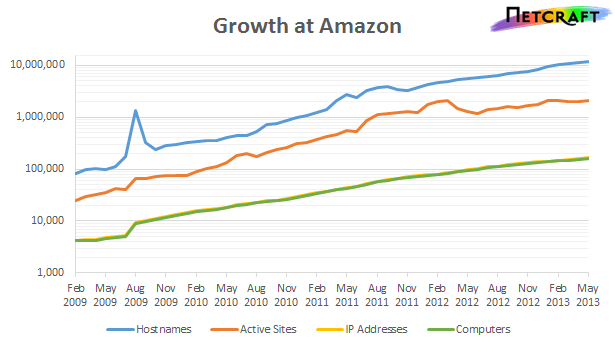
\includegraphics[scale=0.8]{pics/AMZN-growth.png}
	\caption{Croissance chez Amazon\ref{fn1}}
	\label{fig:amazon-growth}
\end{figure}
\bigskip


Ayant tellement nombreux de serveurs en utilisations, le coût généré devient énorme, seulement le coût de consommation d'électricité est déjà considérable. Les fournisseurs sont donc obligés d'optimiser chaque phase de production pour minimiser le coût. 

Avec la technologie de virtualisation, chaque tâche de client est considérée comme une machine virtuelle, plusieurs tâches peuvent s'exécutent en même temps sur une seule machine physique. Alors on a maintenant une question d'ordonnancement: à l'instant donné, quelle tâche doit être exécutée sur quelle machine? Cette question n'est pas facile à répondre à cause de nombreuses contraintes à respecter, qui seront expliquées dans la section suivante.


\section{Description du problème}
Ayant présenté le contexte du problème à traiter, dans cette partie, on va expliquer un peu en détail le problème en introduisant les contraintes à respecter et les objectifs à atteindre. Ils seront décrits d'une façon moins rigoureuse pour être plus compréhensible. La modélisation mathématique du problème peut être trouvée dans le chapitre suivant.


Les tâches seront placées sur des machines connectées en respectant les contraintes suivantes:


\subsection{Contraintes de préaffectation}
Il existe des contraintes qui influence directement sur le résultat de l'ordonnancement:
\bigskip
\begin{enumerate}
	\item Une tâche est planifiée d'être exécutée sur certains instants de temps.
	\item Une tâche ne peut être exécutée que sur certaines machines physiques.
\end{enumerate}
\bigskip

\subsection{Contraintes sur l'utilisation de machines}
Pour héberger une tâche, la machine doit avoir assez de ressources (CPU, GPU, RAM, HDD).


Une tâche peut être migrée d'une machine à l'autre, pendant la migration cette tâche utilise les ressources de toutes ces 2 machines. Puisque la migration est effectuée en parallèle de l'exécution de la tâche sur la machine de source, alors seulement les tâches qui ont été exécutée pendant assez de temps peuvent être migrées.


Une tâche qui est planifiée d'être exécutée peut éventuellement être suspendue si elle est du type préemptable. Pour réveiller cette tâche, il faut d'abord la recharger, ceci va prend du temps.

\subsection{Contraintes sur l'utilisation de réseaux}
Il peut y avoir des affinités entre les tâches. En ce cas, les tâches concernées ont besoin de communiquer entre elles pendant exécution, alors la bande passante du réseau doit être suffisante pour cette communication.



\subsection{Objectifs}
Il y a 2 objectifs à atteindre: minimisation du coût total et minimisation de la durée de reconfiguration.

Pour le premier, voici les coûts qu'on doit considérer:
\bigskip
\begin{itemize}
	\item Le coût d'utilisation des ressources (CPU, GPU, RAM, HDD) de machines.
	\item Le coût de suspension de tâches.
	\item Le coût de rester allumé pour les machines. On peut le considérer comme le coût de consommation. \end{itemize}
\bigskip




\section{Eléments existants}
Dans cette partie on va présenter le travail qui a déjà été réalisé avant ce projet.

\subsection{Modélisation mathématique}
Le modèle mathématique du problème a déjà été créé par Vincent T'Kindt et ses collègues. Toutes les contraintes ainsi que les fonctions objectifs sont déjà représentées sous forme de formulaire. Cette modélisation peut être transmise directement en programme CPLEX, qui peut ensuit trouver la solution optimale.


Le modèle complet peut être trouvé dans le chapitre suivant.

\subsection{Programme de la méthode exacte}
Le programme qui exprime le problème selon le modèle et qui utilise la librairie CPLEX pour trouver la solution optimale a déjà été réalisé par Vincent T'Kindt. Néanmoins, le problème étant prouvé NP-complet, quand on a une grande instance du problème, le programme CPLEX a besoin d'énormément de temps pour trouver une solution. Pour cette raison, on a besoin de chercher une approche heuristique, qui nous permet de trouver très vite une solution assez bonne mais pas forcément optimale.


Même si ce programme CPLEX qui est une approche exacte, n'est peut-être pas très adapté pour les gros instances du problème, il est indispensable dans le test, pour donner la solution optimale qui nous sert ensuite d'évaluer les appoaches heuristiques.


\subsection{Programme de la méthode heuristique}
Une première approche heuristique de liste a été aussi réalisée dans le cadre de PFE (2012 - 2013) de Cyrille PICARD. L'idée de l'approche et les algorithmes concernés ont été decrits dans son rapport de PFE. Par contre, à cause de la complexité du problème et la limite du temps, son implémentation contient des bugs qui rendent le programme incorrect. Alors sur la base de ce programme, j'ai essayé dans un premier temps de corriger les erreurs trouvées et d'améliorer cette implémentation.


\subsection{Programme testeur}
Un testeur a été aussi réalisé par Vincent T'Kindt. Ce testeur contient une partie de génération des instances de problème qui couvre 6 scénarios. Pour chaque instance de problème généré, le testeur appelle le programme de résolution pour trouver la solution et faire des statistiques sur les résultats obtenus.


%\chapter{Mod�le math�matique}
La mod�lisation de ce probl�me a d�j� �t� faite au d�but du projet, mais je la remets ici pour assurer la compl�tude du rapport.

\section{Notions}
Voici un tableau r�capitulatif des notions du probl�me:

\bigskip
\begin{figure}[!htbp]
	\centering
		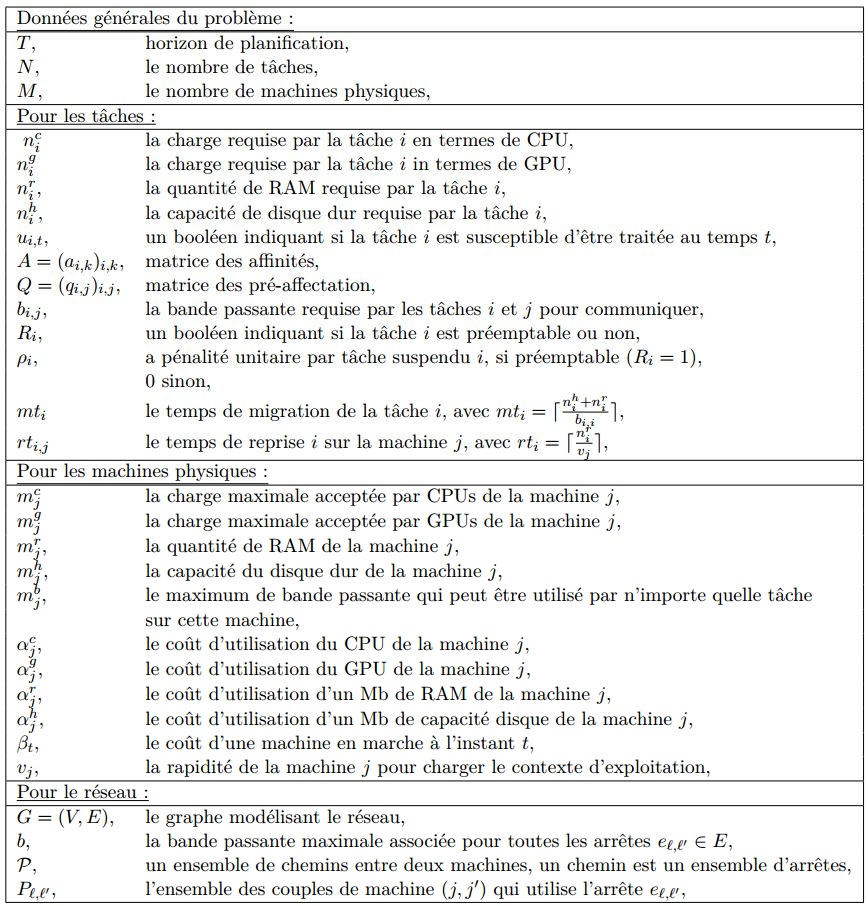
\includegraphics[scale=0.8]{pics/var.jpg}
	\caption{Tableau des variables}
	\label{fig:var}
\end{figure}
\bigskip

\clearpage

\section{Objectifs}
La variable de d�cision du probl�me est la suivante qui repr�sente l'ordonnancement en sortie.

\[
x_{i,t}^{j}=
\left\{ \begin{array}{rl}
			 1 &\mbox{ si la t�che $i$ est trait�e sur la machine $j$ dans l'intervalle $[t, t+1]$} \\
			 0 &\mbox{ sinon}
       \end{array} \right.
\]

On d�finit aussi un ensemble de variables suppl�mentaires suivantes:
\begin{itemize}
	\item $y_{i,i\prime,t}^{j, j\prime} = 1$ si les deux t�ches $i$ et $i\prime$ sont ex�cut�es respectivement sur les machines $j$ et $j\prime$ � l'instant $t$ et ont besoin de communiquer sur le r�seau. Au cas de la migration de t�che $i$ de la machine $j$ vers la machine $j\prime$, $y_{i,i,t}^{j, j\prime} = 1$. Dans les autres cas, on a $y_{i,i\prime,t}^{j, j\prime} = 0$.
	\item $z_{t,j} = 1$ si � l'instant $t$ la machine est en �tat allum�, c'est-�-dire elle ex�cute au moins une t�che en ce moment.
	\item $z_t$ est le nombre de machines en marche � l'instant $t$.
	\item $d_{i,t}$ est la dur�e des op�rations de reconfiguration de la t�che $i$ � l'instant $t$. Ca peut �tre la dur�e d'une op�ration de $resume$ comman�ant � $t$ ou bien la dur�e d'une op�ration de migration terminant � $t$.
\end{itemize}	

Maitenant avec les variables et les notions d�clar�es avant, voici les fonctions objectifs � minimiser.
\begin{eqnarray*}
TC &=& \sum_{t=1}^{T}\sum_{i=1}^{N}\sum_{j=1}^{M}{x_{i,t}^{j}(\alpha_j^cn_i^c + \alpha_j^gn_i^g + \alpha_j^hn_i^h + \alpha_j^rn_i^r)} \\
&+&  \sum_{t=1}^{T}\sum_{i=1}^{N}\sum_{j,k=1; k\neq j}^{M}{y_{i,i,t}^{j,k}(\alpha_k^hn_i^h + \alpha_k^rn_i^r)} \\
&+&  \sum_{t=1}^{T}\sum_{i=1}^{N}(1 - \sum_{j=1}^{M}x_{i,t}^{j})\rho_iu_{i,t}\\
&+&  \sum_{t=1}^{T}{\beta_tz_t}\\
RE &=& \sum_{i=1}^{N}\sum_{t=1}^{T}d_{i,t}
\end{eqnarray*}
\clearpage

\section{Contraintes}
\begin{align} 
 &\sum_{i=1}^{N}{n_i^cx_{i,t}^j} \leq m_j^c  &&\forall t=1,\ldots,T; \nonumber \\
 & &&\forall j=1, \ldots, M     \\
 &\sum_{i=1}^{N}{n_i^gx_{i,t}^j} \leq m_j^g  
  &&\forall t=1,\ldots,T; \nonumber \\
 & &&\forall j=1, \ldots, M        \\                
 &\sum_{i=1}^{N}{n_i^hx_{i,t}^j} + \sum_{j,k=1; k\neq j}^M{n_i^hy_{i,i,t}^{j,k}} \leq m_j^h 
   &&\forall t=1,\ldots,T; \nonumber  \\
  & &&\forall j=1, \ldots, M                   \\    
 &\sum_{i=1}^{N}{n_i^rx_{i,t}^j} + \sum_{j,k=1; k\neq j}^M{n_i^ry_{i,i,t}^{j,k}} \leq m_j^r 
   &&\forall  t=1,\ldots,T; \nonumber \\
  & &&\forall j=1, \ldots, M \\
  %E
  &y_{i,i\prime,t}^{j,j\prime} \geq x_{i,t}^j + x_{i\prime,t}^{j\prime} - 1 
   &&\forall t=1,\ldots,T; \forall i=1, \ldots, N;    \nonumber \\
  & &&\forall i\prime=i+1,\ldots,N dont a_i\prime = 1;  \nonumber \\
  & &&\forall j=1, \ldots, M;  \forall j\prime=j+1, \ldots, M \\
  %F
  &y_{i,i,t}^{j,j\prime} \geq (x_{i,t_1}^j - \sum_{k=1}^M\sum_{t\prime=t_1+1}^{t_2-1}x_{i,t\prime}^k + x_{i,t2}^{j\prime} - 1)
   &&\forall t=1,\ldots,T; \forall i=1, \ldots, N;    \nonumber \\
  & &&\forall j,j\prime=1, \ldots, M et j\neq j\prime;  \nonumber \\
  & &&\forall t_1=t, \ldots, Min(t+mt_i, T) \nonumber \\           
  & &&\forall t_2=t_1+1, \ldots, T \\
  %F'
  &mt_i(x_{i,t}^j - \sum_{k=1}^M\sum_{t\prime=t+1}^{t_1-1}x_{i,t\prime}^k + x_{i,t_1}^{j\prime} - 1) \leq \sum_{t\prime=max(t+1-mt_i, 0)}^tx_{i,t}^j 
   &&\forall t=1,\ldots,T; \forall i=1, \ldots, N;    \nonumber \\
  & &&\forall j,j\prime=1, \ldots, M et j\neq j\prime;  \nonumber \\
  & &&\forall t_1=t+1, \ldots, T \\
  %G
  &\sum_{j=1}^Mx_{i,t}^j = u_{i,t}  &&\forall i=1, \ldots, N, dont R_i=0; \nonumber \\
  & &&\forall t=1,\ldots,T \\
  %H
  &\sum_{j=1}^Mx_{i,t}^j \leq u_{i,t} 
   &&\forall i=1, \ldots, N, dont R_i=1; \nonumber \\
  & &&\forall t=1,\ldots,T \\
  %I
  &x_{i,t}^j \leq u_{i,t}q_{i,j} 
   &&\forall t=1,\ldots,T; \forall i=1, \ldots, N;    \nonumber \\
  & &&\forall j=1, \ldots, M \\
  %J
  &\sum_{(j,j\prime)\in P_{l,l\prime}, j<j\prime}(
   \sum_{i,i\prime=1, i<i\prime, a_{i,i\prime}=1}^N b_{i, i\prime}y_{i,i\prime,t}^{j,j\prime}
   + \sum_i^N b_{i, i}(y_{i,i,t}^{j,j\prime} + y_{i,i,t}^{j\prime,j})
  ) \leq b \nonumber \\
  & &&\forall t=1,\ldots,T; \forall e_{l,l\prime}\in E 
\end{align}
\clearpage
\begin{align}
	%K
  &z_{t,j} \geq x_{i,t}^j 
   &&\forall t=1,\ldots,T; \forall i=1, \ldots, N;    \nonumber \\
  & &&\forall j=1, \ldots, M \\  
  %L
  &z_{t} = \sum_{j=1}^Mz_{t,j} &&\forall t=1,\ldots,T \\
  %M
  &x_{i,t_2}^j \leq 1 - x_{i,t_1}^j + x_{i,t_1+1}^j  
   &&\forall i=1, \ldots, N, dont R_i=1;    \nonumber \\
  & &&\forall j=1, \ldots, M;  \nonumber \\
  & &&\forall t_1=1, \ldots, T-rt_{i,j}; \nonumber \\           
  & &&\forall t_2=t_1+1, \ldots, t_1+rt_{i,j} \\
  %N
  &d_{i,t_1} \geq (t_2 - t_1)(x_{i,t_1-1}^j - \sum_{k=1}^M\sum_{t=t_1}^{t_2-1}x_{i,t}^k - 1 + x_{i,t_2}^j)
   &&\forall i=1, \ldots, N, dont R_i=1;    \nonumber \\
  & &&\forall j=1, \ldots, M;  \nonumber \\
  & &&\forall t_1=1, \ldots, (T-rt_{i,j}-1); \nonumber \\           
  & &&\forall t_2=t_1+rt_{i,j}+1, \ldots, T \\
  %O
  &d_{i,t_1} \geq mt_i(x_{i,t_1}^j  + x_{i,t_1+1}^{j\prime} -1)  &&\forall i=1, \ldots, N;    \nonumber \\
  & &&\forall j,k=1, \ldots, M, j\neq k;  \nonumber \\
  & &&\forall t_1=1, \ldots, (T-mt_i-1); \nonumber \\           
  & &&\forall t_2=t_1+mt_i+1, \ldots, T
\end{align}

%\chapter{Planification du projet}

\section{D�coupage des t�ches}
Ce projet consiste globalement � 5 t�ches � r�aliser, qui sont d�crits au-dessous.
\bigskip
\begin{itemize}
	\item Corriger et am�liorer la m�thode heuristique.
	\item R�aliser une m�thode heuristique bas�e sur le solveur CPLEX.
	\item Effectuer des recherches sur le pr�traitement du mod�le de probl�me pour am�liorer le fonctionnement de la m�thode exacte.
	\item Effectuer des campagnes de tests.
	\item Analyser et comparer les r�sultats obtenus.
	\item D�velopper de nouvelles m�thodes de r�solution.
\end{itemize}
\bigskip

\subsection{Reprise de l'existant}
Cette premi�re t�che consist � �tudier le probl�me et reprendre les travaux qui ont d�j� �t� effectu�s. C'est la t�che de base pour la suite du projet.

\subsection{Am�lioration et compl�tion du programme heuristique}
Parmi les travaux d�j� r�alis�s, l'impl�mentation de l'algorithme heuristique reste � �tre corrig� et am�lior�. La deuxi�me t�che du projet est alors de modifier le code pour faire fonctionner correctement ce programme heuristique.

\subsection{Lancement de tests et de comparaison}
Apr�s avoir fini la modification du programme heuristique, il faut faire le test � l'aide du programme Testeur. Ensuite il faut comparer les r�sultats donn�s par l'heuristique et les r�sultats donn�s par la m�thode exacte. Les aspects � comparer comprennent le nombre d'instances r�solu, le temps d'ex�cution pour trouver la solution et la d�viation entre les r�sultats, etc.

\subsection{R�alisation de la seconde m�thode heuristique}
Cette t�che est ajout�e au mi-cours du projet. L'id�e est d'ajouter des caract�ristiques heuristiques dans la m�thode exacte pour avoir un meilleur compromis entre la qualit� du r�sultat et le temps d�pens� pour chercher la solution.

Pour le faire, on va mettre en place des param�tres CPLEX pour bien contr�ler le temps d'ex�cution. Par exemple on peut arr�ter le programme au bout de 3 minutes d'ex�cution, ou bien on peut l'arr�ter quand on est s�r que la solution actuelle a au moins 95\% de qualit� par rapport � la solution optimale, etc. 

\subsection{Recherche sur le pr�traitement des donn�es pour la m�thode exacte}
Cette t�che est la partie principale du projet. On va travail cette fois sur la m�thode exacte. L'id�e est de faire des pr�traitements des donn�es d'entr�e du programme exact, pour que ce dernier peut trouver plus facilement la solution optimale avec ces donn�es pr�trait�es. Il s'agit du travail collaboratif avec d'autres chercheurs. 

\section{Planning}
Cette partie concerne le planning des t�ches. Cependant en tant que projet de type recherche, ce n'est pas �vident d'�valuer la dur�e des t�ches. Ici cen'est un planning en g�n�ral, ceci peut �voluer suivant le d�roulement du projet.

\subsection{Diagramme Gantt}
\bigskip
\begin{figure}[!htbp]
	\centering
		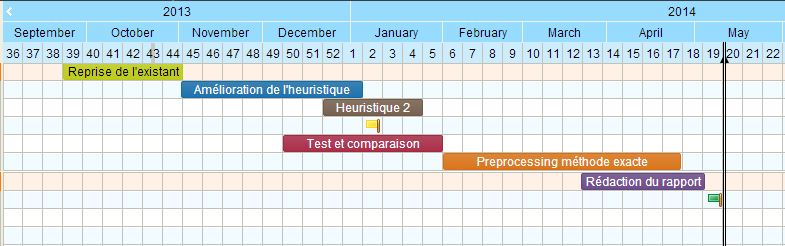
\includegraphics{pics/gantt.JPG}
	\caption{Diagramme de Gantt}
	\label{fig:gantt}
\end{figure}
\bigskip


%\documentclass[twoside,fleqn]{EPURapport}
%\usepackage{listings}
\usepackage[french]{algorithm2e}
\usepackage{caption}
%\renewcommand{\lstlistlistingname}{Liste des codes}
%\renewcommand{\lstlistingname}{Code}

%\addextratables{%
%	\lstlistoflistings
%}

%\swapAuthorsAndSupervisors


\usepackage{hyperref}
\usepackage{amsmath}
\usepackage{ulem}
\usepackage[utf8]{inputenc}
%\usepackage{todonotes}

%\nolistoftables
%\thedocument{Rapport PFE}{Résolution d'un problème off-line de consolidation de serveurs}{}
\thedocument{Rapport des Tests}{Rapport des tests du problème SCP (hors-ligne)}{}

\grade{Département Informatique\\ 5\ieme{} année\\ 2013 - 2014}
\authors{%
	\category{Étudiants}{%
		\name{Lei SHANG} \mail{lei.shang@etu.univ-tours.fr}
	}
	\details{DI5 2013 - 2014}
}

\supervisors{%
	\category{Encadrants}{%
		\name{Vincent T'Kindt} \mail{vincent.tkindt@univ-tours.fr}
	}
	\details{Université François-Rabelais, Tours}
}

\abstracts{}{}


\renewcommand{\theequation}{\Alph{equation}}	
\begin{document}

%%%
%%% Cuts
%%%
\chapter{Valide inequalities}
\section{Cuts classiques}
Les Cuts classiques sont des coupes qui ne dépendent pas la particularité du problème. Nous présentons dans cette section qu'un seul type de coupes: 1-Cuts.
\subsection{1-Cuts}\label{cut2}
1-cuts par Osorio et al.(2002) sont des coupes générées à partir des contraintes de types $d^Tx \leq b$ avec $d_1  \geq d_2 \geq \dots \geq d_n > 0$. Ce sont donc des contraintes redondantes qui peut pourtant plus efficaces. Par exemple pour la contrainte $x_1+2x_2+2x_3\leq 3 \ $dont les variables sont binaires, on peut en déduire un 1-cuts $x_2+x_3 < 1$, car si $x_2 = x_3=1$ la contrainte originale sera violée.

Il existe déjà l'algorithme\cite{t2007enumeration} pour générer automatiquement les 1-cuts, alors nous l'avons réalisé et ensuite appliqué sur les contraintes de ressources dans le Preprocessing. Le résultat de test montre que ces coupes ont bien un effet possitif pour fixer plus de variables surtout pour les permiers 3 scénarios. Cependant, nous avons aussi aperçu que le nombre de coupes générées est considérable pendant cette démarche, ce qui peut potentiellement avoir un effet négatif sur le temps de résolution, parce que quand nous avons de nombreux contraintes ajoutés, Cplex va alors mettre plus de temps pour traiter ces contraintes.

Pour résoudre ce problème, nous nous posons la question: combien de 1-cuts devons nous générer et quelles sont les contraintes prioritaires. Empiriquement, nous décitons de trier les contraintes par ordre croissante de la partie droite de l'équation (noté $RHS$) car quand le $RHS$ est plus petit, ça génère des coupes plus contraignant. Après, en considérant la partie gauche de l'équation, nous avons aussi essayé une deuxième approche, c'est de trier les contraintes par ordre décroissante de $LRS/RHS$, dont $LRS$ est la somme des coefficients à gauche de l'équation.

Pour la question sur le nombre de coupes à générer, nous avons fait un test sur des instances choisies avec un nombre différent des coupes pour voir c'est combien le seuil pour chaque scénario. Ensuite avec le résultat des scénarios 4, 5 et 6 comme échantillons, nous avons trouvé une fonction qui peut donner un seuil selon le nombre de tâche et le nombre de machine du problème. La recherche de cette fonction est basé sur la procédure de "Multiple Linear Regression". Un outil en ligne\footnote{\url{http://www.xuru.org/rt/MLR.asp}} a été utilisé pour cette recherche.

Les différents tests effectués sont décrits dans les chapitres suivants.

\section{Cuts problème-dépendent}
\subsection{Cuts sur les contraintes des ressources}\label{cut1}
\subsubsection{Ressources CPU/GPU}
Si la tâche $i$ ne peut pas être affectée au serveur $j$ à cause de la capacité résiduelle de CPU/GPU du serveur, alors pour toute les tâches qui demandent plus de CPU/GPU que la tâche $i$, cette affectation ne peut pas être effectuée non plus.


Cette contrainte peut être exprimée de façon suivante:
\bigskip

%CPU
$Si \  n^c_{i\prime}\geq n^c_{i}\ alors\;$
\begin{align} 
&x_{i,j,t}+x_{i\prime,j,t}\leq (m^c_j-\sum^N_{k=1; k\neq{i},i\prime;u_{k,t}=q_{k,j}=1}{n^c_kx_{k,j,t}})/n^c_i
&&\forall t=1,\ldots,T, tq\ u_{i,t}=u_{i\prime,t}=1; \nonumber \\
 & &&\forall j=1, \ldots, M, tq\ q_{i,j}=q_{i\prime,j}=1
\end{align} 
 
%GPU
$Si\ n^g_{i\prime}\geq n^g_{i}\ alors\;$
\begin{align} 
&x_{i,j,t}+x_{i\prime,j,t}\leq (m^g_j-\sum^N_{k=1; k\neq{i},i\prime;u_{k,t}=q_{k,j}=1}{n^g_kx_{k,j,t}})/n^g_i 
&&\forall t=1,\ldots,T, tq\ u_{i,t}=u_{i\prime,t}=1; \nonumber \\
 & &&\forall j=1, \ldots, M, tq\ q_{i,j}=q_{i\prime,j}=1
\end{align} 


À noter que nous n'avons pas besoin de considérer ici la contraite de préaffectation.

\subsubsection{Ressources HDD/RAM}
Les cuts sur les ressources HDD/RAM ont le même principe sauf que ces ressources puissent aussi être occupées par l'opération de la migration. Nous pouvons appliquer les mêmes cuts comme pour CPU/GPU mais la prise en compte de la migration peut rendre le cut plus strict.
\bigskip

%HDD
$Si\ n^h_{i\prime}\geq n^h_{i}\ alors\;$
\begin{align}
x_{i,j,t}+x_{i\prime,j,t} &\leq (m^h_j-\sum^N_{k=1;k\neq{i},i\prime;u_{k,t}= q_{k,j}=1}{n^h_kx_{k,j,t}} \nonumber \\
 & - \sum^N_{k=1; k\neq{i},i\prime}{\sum^M_{l=1;l\neq{j}}{n^h_ky^{l,j}_{k,k,t}} }\;)/n^h_i        &&\forall t=1,\ldots,T, tq\ u_{i,t}=u_{i\prime,t}=1;  \nonumber \\
 & &&\forall j=1, \ldots, M, tq\ q_{i,j}=q_{i\prime,j}=1
\end{align}

%RAM
$Si\ n^r_{i\prime}\geq n^r_{i}\ alors\;$
\begin{align}
x_{i,j,t}+x_{i\prime,j,t} &\leq (m^r_j-\sum^N_{k=1;k\neq{i},i\prime;u_{k,t}= q_{k,j}=1}{n^r_kx_{k,j,t}} \nonumber \\
 & - \sum^N_{k=1; k\neq{i},i\prime}{\sum^M_{l=1;l\neq{j}}{n^r_ky^{l,j}_{k,k,t}} }\;)/n^r_i        &&\forall t=1,\ldots,T, tq\ u_{i,t}=u_{i\prime,t}=1;  \nonumber \\
 & &&\forall j=1, \ldots, M, tq\ q_{i,j}=q_{i\prime,j}=1
\end{align}


\subsection{Machines équivalentes* (incorrect, à enlever)}
Deux serveurs $j$ et $j'$ peut être totalement identique dans une instance de problème si:
\begin{enumerate}
\item Les caractéristiques (CPU/GPU/HDD/RAM) de $j$ et $j'$ sont identiques
\item $q_{i,j} = q'_{i,j}$ pour $\forall i$
\item \sout{$j$ et $j'$ ont les même voisins dans le réseau}
\item \sout{Pour chaque voisin $v$ de $j$ (et $j'$), la bande passante entre $v$ et $j$ est la même que celle entre $v$ et $j'$}
\end{enumerate}
\bigskip
\sout{Plus largement, le $j$ et $j'$ ci-dessus peuvent être considérés comme un sous-réseau mais pas simplement un seul serveur. Comme ça, étant donné une solution, on peut très bien construir une autre en échangeant les affectation en $j$ et $j'$.}

[Update]Après étude du réseau, il parâit que toutes les machines sont connectées et la bande passante est unique donc on n'a besoin que de considérer les deux premières conditions. [Update]Mais quand même, si l'affectation ne se fait pas au premier instant, c'est possible que l'environnement réseau des machines équivalentes devient différent.

Si $j$ et $j'$ sont deux machines identiques alors pour le premier instant de temps où il y a des tâches qui s'exécutent sur $j$ ou $j'$, alors on peut forcer que le serveur $j$ est plus utilisé que $j'$ pour éliminer les solutions redondantes:
\begin{align}
\sum_{t_1=1}^{t-1}\sum_{i_1=1}^{N}x_{i_1,j,t_1}+ CPUUsed(j,t)-CPUUsed(j',t) \geq 0
 && \forall t=1,\ldots,T;   \nonumber \\
 && \forall j,j'=1\ldots M, j<j', \nonumber \\
 && équivalent(j,j');
\end{align}
[Update]C'est faux! On ne doit pas utiliser la différence des CPUUsed dans le formule car cette différence n'est pas binaire, donc même si $\sum_{t_1=1}^{t-1}\sum_{i_1=1}^{N}x_{i_1,j,t_1} \geq 0$, cette contrainte est quand même fonctionnelle.

\subsection{Dominance des tâches* (à enlever)}
Cette fois on va prendre en compte toutes les ressources requises par la tâche. On modélise 2 tâches $i$ et $i\prime$ pour que la tâche $i\prime$ a besoin de plus de ressource que $i$ pour tout type de ressources y compris la partie du réseau.

La formulation courante de ce cut n'est peut-être pas valide, parce que même si nous avons $x_{i,j,t}=0$ ça ne veut pas dire qu'il n'y a pas de ressources pour la tâche $i$. Ça peut simplement parce que $x_{i,j,t}=1$ ne conduit pas à la solution optimale.

Alors si nous voulons créer un Cut sur les ressources du réseau, je pense c'est quand même mieux de reprendre le même principe: si on est sûr que les ressources réseau sont insuffisantes pour la tâche $i$ alors c'est pareil pour $i\prime$. Cependant cette modélisation (état de l'insuffisance de ressources) ne me semble pas évidente.

%%%
%%% Test sans preprocessing
%%%
\chapter{Test des méthodes de résolution sans Preprocessing}
Pour tester le fonctionnement des différentes méthodes de résolution dans ce projet, plusieurs tests ont été effectués sur un ensemble d'instances du problème. Cet ensemble contient 6 scénarios dont chacun est composé par 20 instances du problème. Toutes ces données de test sont générées par le programme Testeur.


\section{Méthode exacte - solveur Cplex}
Dans un premier temps, le test du solveur Cplex est effectué car les solutions trouvées par le solveur peuvent nous servir à évaluer la performance des autres méthodes de résolution.

Le tableau \ref{tab_cplex} représente les statistiques effectuées sur le résultat de test du solveur Cplex. Les significations des colonnes sont:
\begin{enumerate}
	\item Sc(N/M): numéro de scénario et le nombre de VM et de serveur physique.
	\item \#Infeas: le nombre des instances qui sont prouvées comme ''Infaisable'' par le solveur.
	\item \#Opt: le nombre des instances qui sont résolues avec la solution optimale trouvée.
	\item \#Mem: le nombre des instances pour lesquelles le solveur n'a pas pu trouver la solution optimale à cause de la limite de l'espace mémoire.
	\item \#Tim: le nombre des instances pour lesquelles le solveur n'a pas pu trouver la solution optimale à cause de la limite du temps.
	\item $T_{min}$, $T_{avg}$, $T_{max}$: le temps (minimum, moyenne et maximum) de résolution en seconde.
\end{enumerate}
\bigskip

\begin{table}[h]
    \centering
    \begin{tabular}{|c|c|c|c|c|c|c|c|}
    	\hline
    	Sc(N/M)	& \#Infeas & \#Opt	& \#Mem & \#Tim & $T_{min}$ & $T_{avg}$	& $T_{max}$ \\ \hline
		Sc1(8/2) & 2 & 18 & 0 & 0 &  0.02 &  0.07 &  0.15 \\ \hline
		Sc2(11/3) & 9 & 11 & 0 & 0 &  0.08 &  0.34 &  1.08 \\ \hline
		Sc3(15/4) & 1 & 19 & 0 & 0 &  0.59 &  4.33 &  54.57 \\ \hline
		Sc4(18/5) & 0 & 19 & 0 & 1 &  1.88 &  239.53 &  1800.37 \\ \hline
		Sc5(21/5) & 3 & 6 & 1 & 10 &  1.68 &  1196.57 &  1800.74 \\ \hline
		Sc6(24/6) & 2 & 5 & 0 & 13 &  2.06 &  1316.75 &  1820.14 \\	\hline
    \end{tabular}
    \caption{Résultat de test du solveur Cplex}
    \label{tab_cplex}
\end{table}
\bigskip

A partir du scénario 4, on commence à avoir des grosses instances pour lesquelles le solveur n'a pas pu trouver la solution optimale ($T_{max}=1800$) à cause de la limite de temps.

\section{Méthode heuristique de liste}
Le tableau \ref{tab_h1} montre le résultat de test de la méthode heuristique de liste (on l'appelle H1 pour raison de simplicité). Dans ce tableau, les colonnes $D_{min}$, $D_{avg}$ et $D_{max}$ signifient la déviation entre la solution trouvée par H1 et la solution trouvée par le solveur Cplex. A noter que pour les 3 premiers scénarios le solveur a trouvé la solution optimale pour toutes les instances donc cette déviation peut montrer la qualité de notre méthode H1 par rapport à la solution optimale. A partir du scénario 4 on commence à avoir des instances pour lesquelles le solveur a trouvé une solution faisable mais pas optimale à cause de la limite du temps ou de l'espace mémoire, alors dans ce cas la déviation est aussi affectée.


\begin{table}[h]
    \centering
    \begin{tabular}{|c|c|c|c|c|c|c|c|c|}
    	\hline
    	Sc(N/M)	& \#Infeas & \#Solved	& $T_{min}$ & $T_{avg}$	& $T_{max}$ & $D_{min}$ & $D_{avg}$	& $D_{max}$ \\ \hline
		Sc1(8/2)  & 2 & 18 & 0.00 & 0.00 & 0.00 &0\% &19\% &67\% \\ \hline
Sc2(11/3) & 9 & 11 & 0.00 & 0.00 & 0.00 &0\% &17\% &46\% \\ \hline
Sc3(15/4) & 7 & 13 & 0.00 & 0.00 & 0.00 &5\% &24\% &58\% \\ \hline
Sc4(18/5) & 11 & 9 & 0.00 & 0.00 & 0.00 &10\%& 27\%& 37\% \\ \hline
Sc5(21/5) & 16 & 4 & 0.00 & 0.00 & 0.01 &30\%& 36\%& 43\% \\ \hline
Sc6(24/6) & 20 & 0 & 0.00 & 0.01 & 0.02 & * & * & * \\ \hline
    \end{tabular}
    \caption{Résultat de test de la méthode heuristique de liste (H1)}
    \label{tab_h1}
\end{table}
\bigskip

On trouve souvent 0.00 seconde dans les colonnes de temps, ce qui signifie que le temps de résolution de H1 est très court.


Par rapport à la déviation, la performance de H1 n'est pas très stable: pour certaines instances du problème, H1 a trouvé la solution optimale ($D_{min}=0\%$) mais on a aussi dans le Sc1 $D_{max}=67\%$ qui n'est pas très optimiste. Pour le scénario 6, H1 n'a résolu aucune instance donc la déviation n'est pas calculée.


\section{Méthode heuristique de Cplex}
Le tableau \ref{tab_h2} montre le résulat de test sur la méthode heuristique basée sur le solveur Cplex (H2).


\begin{table}[h]
    \centering
    \begin{tabular}{|c|c|c|c|c|c|c|c|c|}
    	\hline
    	Sc(N/M)	& \#Infeas & \#Solved	& $T_{min}$ & $T_{avg}$	& $T_{max}$ & $D_{min}$ & $D_{avg}$	& $D_{max}$ \\ \hline
		Sc1(8/2)  &2 & 18 &  0.02 &  0.07   &0.15     &0\%  &0\%  &1\% \\ \hline
Sc2(11/3) &9 & 11 &  0.08 &  0.29   &0.97     &0\%  &0\%  &1\% \\ \hline
Sc3(15/4) &1 & 19 &  0.64 &  1.37   &5.21     &0\%  &0\%  &2\% \\ \hline
Sc4(18/5) &0 & 20 &  1.53 &  80.33  & 400.32  &0\%  &0\%  &2\% \\ \hline
Sc5(21/5) &3 & 17 &  1.68 &  240.31 &  400.41 & 0\% & 2\% & 4\% \\ \hline
Sc6(24/6) &2 & 18 &  2.08 &  286.79 &  410.43 & -1\%&  1\%&  7\% \\ \hline
    \end{tabular}
    \caption{Résultat de test de la méthode heuristique de Cplex (H2)}
    \label{tab_h2}
\end{table}
\bigskip


Puisque la méthode H2 est basée sur le solveur Cplex, pour les petites instances de problème elle a trouvé des solutions qui sont très proches des solutions optimales. Pour les grandes instances (à partir du scénario 4), les solutions qu'elle a trouvées sont aussi très intéressantes avec la déviation maximale égale à 7\% qui reste acceptable. Le temps maximum de résolution est vers 200 secondes qui provient de l'implémentation de H2.



%%%
%%% Preprocessing
%%%
\chapter{Test du Preprocessing} 
Un autre ensemble de tests a été réalisé pour évaluer la performance de l'approche Preprocessing avec des coupes différentes.

On rappelle ici l'idée du Preprocessing est de fixer autant que possible de variables dans le modèle pour réduire la taille du problème. Pour le faire, il faut avoir une borne supérieure (UB) et une borne inférieure (LB) qui sont assez proches de la solution optimale.

\section{Preprocessing sans coupes supplémentaires}
Nous avons lancé d'abord le Preprocessing sur toutes les variables booléennes sans ajoutant des coupes supplémentaires.

Dans le tableau \ref{tab_pre} on peut trouver des statistiques sur la qualité des LB et des UB ainsi que la proportion de variables fixées pendant le Preprocessing. Les colonnes s'interprêtent comme le suivant:
\begin{enumerate}
	\item DevLB: la déviation (minimum, moyenne et maximum) entre la solution optimale et LB.
	\item DevUB: la déviation (minimum, moyenne et maximum) entre UB et la solution optimale.
	\item Fixed: la proportion du nombre de variables fixées par rapport au nombre de toutes les variables ayant passé le preprocessing.
\end{enumerate}

\bigskip
\begin{table}[h]
    \centering
    \begin{tabular}{|c|c|c|c|c|c|c|c|c|c|}
    	\hline 
    	&\multicolumn{3}{c|}{DevLB}& \multicolumn{3}{c|}{DevUB}& \multicolumn{3}{c|}{Fixed} 	\\ \hline
    	Sc(N/M)	& min & avg & max & min & avg & max & min & avg & max\\ \hline
Sc1(8/2) & 0.00\%  &4.83\%  &17.07\%  &0.00\% & 0.04\%  &0.65\%  &0.00\%  &9.25\% &51.83\% \\ \hline
Sc2(11/3)&  0.04\% & 7.21\% & 17.13\% & 0.00\%&  0.01\% & 0.15\% & 0.00\% &13.90\% & 66.67\%\\ \hline
Sc3(15/4)&  1.10\% & 4.01\% & 10.12\% & 0.00\%&  0.36\% & 1.80\% & 0.00\% &0.88\% & 10.96\%\\ \hline
Sc4(18/5)&  0.05\% & 5.28\% & 12.56\% & 0.00\%&  0.53\% & 1.81\% & 0.00\% &2.86\% & 55.64\%\\ \hline
Sc5(21/5)&  1.82\% & 5.03\% & 8.94\%  &0.56\% & 1.94\%  &7.62\%  &0.00\%  &0.00\% &0.00\%\\ \hline
Sc6(24/6)&  3.94\% & 5.91\% & 8.72\%  &0.30\% & 1.75\%  &5.40\%  &0.00\%  &0.09\% &0.56\%\\ \hline
    \end{tabular}
    \caption{Résultat de test du Preprocessing sur toute les variables booléannes}
    \label{tab_pre}
\end{table}
\bigskip
Nous constatons que le Preprocessing naïf fonctionne mais pas suffisamment bien. Il ne fixe pas beaucoup de variables donc il n'aide pas la résolution de Cplex. Souvent, ce problème survient quand l'UB ou LB n'est pas assez bonne. En comparant la qualité de LB et de UB, on peut trouver que relativement les UB sont assez proches que la solution optimale, en revanche les LB ne sont pas très bonnes.

Pour améliorer les LB, nous avons cherché d'ajouter des contraintes supplémentaires (Cuts) au modèle LP du problème, pour enfin améliorer le fonctionnement du Preprocessing.

\begin{comment}
\subsubsection{Preprocessing sur les variables booléennes de décision $X^t_{i,j}$}
Le tableau \ref{tab_pre_x} est le résultat d'un autre test sur Preprocessing. Dans ce test, au lieu de passer toutes les variables au Preprocessing, on passe seulement les variables de décision $X^t_{i,j}$, qui représente l'ordonnancement trouvé, au Preprocessing car on pense que ces variables sont les plus influentes. Par rapport au premier test, ce test ne change que les 3 dernières colonnes sur la proportion des variables fixées, le résultat sur la qualité de LB et UB reste le même.


\begin{table}[h]
    \centering
    \begin{tabular}{|c|c|c|c|}
    	\hline
    	Sc(N/M)	&  $Fix_{min}$ & $Fix_{avg}$ & $Fix_{max}$\\ \hline
    	Sc1(8/2) &0.00\% & 13.84\% & 100.00\%\\ \hline
Sc2(11/3)&0.00\% & 10.15\% & 42.42\%\\ \hline
Sc3(15/4)&0.00\% & 0.56\%  &7.36\%\\ \hline
Sc4(18/5)&0.00\% & 3.07\%  &59.07\%\\ \hline
Sc5(21/5)&0.00\% & 0.00\%  &0.00\%\\ \hline
Sc6(24/6)&0.00\% & 3.45\%  &59.07\%\\ \hline
    \end{tabular}
    \label{tab_pre_x}
    \caption{Résultat de test du Preprocessing sur les variables de décision $X^t_{i,j}$}
\end{table}
\bigskip

\subsection{Conclusion sur le Preprocessing}
En comparant le résultat détaillé des deux tests effectués, on a constaté que la plupart des variables fixées sont les variables de décision $X^t_{i,j}$. Cependant, pour certaines instances, si on passe seulement les $X^t_{i,j}$ au Preprocessing aucune variable peut être fixée mais si on passe toutes variables booléennes au Preprocessing il y aura des variables fixées. Ça veut dire il y a quand même des variables booléennes qui ne sont pas $X^t_{i,j}$ mais qui ont des effets sur le Preprocessing. En conclusion on pense que c'est mieux de faire le Preprocessin pour toutes les variables booléennes.

\end{comment}

\section{Preprocessing avec coupe 1}
Nous avons d'abord relancé le test de Preprocessing avec la coupe 1 (cf \ref{cut1}) qui est problème-dépendant concernant les contraintes de ressources. Malheureusement, l'ajout de cette coupe n'a apporté aucun changement au résulat de test (identique que \ref{tab_pre}). Nous pouvons donc dire que la coupe 1 n'est pas utile pour le fixage des variables pendant le Preprocessing, mais c'est très probable qu'elle est efficace dans le MIP. Néanmoins, à cause de la limite de temps, nous n'avons pas pu tester la performance de cette coupe dans le MIP.


\section{Preprocessing avec coupe 2}
Cette partie contient le résultat (tableau\ref{tab_pre_2}) de test de Preprocessing avec la coupe 2 (aussi notée 1-Cuts, cf \ref{cut2}).
\begin{table}[h]
    \centering
    \begin{tabular}{|c|c|c|c|c|c|c|c|c|c|}
    	\hline
&\multicolumn{3}{c|}{DevLB}& \multicolumn{3}{c|}{DevUB}& \multicolumn{3}{c|}{Fixed} 	\\ \hline
    	Sc(N/M)	& min & avg & max & min & avg & max & min & avg & max\\ \hline
Sc1(8/2) & 0.00 \% &	2.87\%  &	17.07	\%  &0.00\% & 0.04\%  &0.65\%  &0.00\%  &43.91	\% &100.00\% \\ \hline
Sc2(11/3)& 0.04 \% & 	4.54\% & 	11.97	\% & 0.00\%&  0.01\% & 0.15\% & 0.00\%  &15.80	\% &66.67\%\\ \hline
Sc3(15/4)& 0.44 \% & 	3.47\% & 	9.40	\% & 0.00\%&  0.36\% & 1.80\% & 0.00\%  &2.22	\% &10.96\%\\ \hline
Sc4(18/5)& 0.05 \% & 	4.94\% & 	11.60	\% & 0.00\%&  0.53\% & 1.81\% & 0.00\%  &2.91	\% &55.64\%\\ \hline
Sc5(21/5)& 1.82 \% & 	4.72\% & 	8.82	\%  &0.56\% & 1.94\%  &7.62\%  &0.00\%  &0.00	\% &0.00\%\\ \hline
Sc6(24/6)& 3.64 \% & 	5.65\% & 	8.45	\%  &0.30\% & 1.75\%  &5.40\%  &0.00\%  &0.09	\% &0.56\%\\ \hline 
    \end{tabular}
    \caption{Résultat de test du Preprocessing avec la coupe 2}
    \label{tab_pre_2}
\end{table}
\bigskip


Dans le résultat, les trois colonnes de UB restent les mêmes car le Preprocessing n'affecte que sur les LB. Nous pouvons trouver que avec la coupe 2, le Preprocessing a pu fixé plus de variables qu'avant, surtout pour les premiers 3 scénarios. En conséquence, les LB ont été aussi améliorées (la déviation entre la solution optimale et la LB devient plus petite).

En résumé, la coupe 2 est utile pour renforcer le Preprocessing mais le résultat n'est pas encore assez bon pour bien accélérer la résolution après. A partir de scénario 4, le Preprocessing n'aide quasiment plus.

\section{Preprocessing avec coupe 1\&2* (à enlever, peut-être)}
Le résultat du test de Preprocessing avec à la fois la coupe 1 et la coupe 2 reste pareil que le Preprocessing avec la coupe 2 seule (\ref{tab_pre_2}). Ce fait a confirmé que la coupe 1 n'est pas utile pour le fixage des variables.


\section{Preprocessing avec la coupe 2 renforcée}
Selon les tests que nous avons fait, la coupe 2 a des effects positifs pour le Preprocessing. Nous avons donc effectué des démarches pour encore renforcer la coupe 2.

Dans la phase de fixage, le Preprocessing peut fixer des variables en générant des contraintes, mais quand le nombre de contraintes devient plus en plus grand, ça peut au contraire ralentir la résolution de Cplex dans la phase suivante. Dans notre cas, puisque la coupe 2 va générer beaucoup de contraintes, nous essayons donc de trouver un seuil supérieur pour le nombre des contraintes générés. Mise en place de ce paramètre doit diminuler autant que possible le temps utilisé pour la résolution MIP, tout en assurant que le nombre de variables fixées ne soit pas diminué.

Pour trouver la relation entre le nombre de contraites générées à partir de la coupe 2 et le temps dépensé pendant la résolution Cplex, nous avons conçu deux tests d'analyse.
\subsubsection{Premier test de l'analyse du nombre de coupes à générer}
Les principles du premier test sont:
\begin{enumerate}
	\item Pour chacun des scénarios 4, 5 et 6, nous choisissons 5 instances de problème qui peuvent être résolues à l'optimalité dans un temps modéré (pas trop court pour être observable ni trop long pour ne pas dépasser la limite de temps).
	\item Pour chaque instance, nous faisons un série de tests avec un seuil de nombre de coupes différents. Ce seuil commence à 200 puis s'incrémente d'un pas de 200 jusqu'à le nombre total des coupes qu'on peut générer.
	\item Après le test, pour chaque scénario, nous cherchons le seuil qui donne un temps moyen d'exécution minimum pour les 5 instances choisies.
	\item Pour que les coupes générées soient les plus contraignantes, nous avons trier avant la génération de coupe 2, les contraintes en ordre croissante de RHS (cf \ref{cut2}).
\end{enumerate}
	
Le résultat du test (tableau\ref{tab_pre_2_seuil}) nous a donné des échantillons pour étudier la corrélation entre le meilleur seuil et les caractéristiques de scénarios.

\begin{table}[h]
    \centering
    \begin{tabular}{|c|c|c|c|}
    	\hline
Sc& 	N	& M	& BestSeuil\\ \hline
4 & 	18	& 5	& 600      \\ \hline
5 & 	21	& 5	& 400      \\ \hline
6 & 	24	& 6	& 1600     \\ \hline
    \end{tabular}
    \caption{Résultat du premier test d'analyse du seuil de la coupe 2}
    \label{tab_pre_2_seuil}
\end{table}
\bigskip

Ce résultat montre que quand N (le nombre de tâches) augmente, BestSeuil diminue et quand M (le nombre de machines) augmente, BestSeuil augmente. Empiriquement, nous avons fait une "Multiple Linear Regression"\footnote{\url{http://www.xuru.org/mlr}} sur ces données de test pour trouver une fonction qui peut donner le meilleur seuil pour un scénario. Le fonction trouvée (notée Seuil1) est:
\begin{align}
BestSeuil=-66.67N+1400M-5200
\end{align}

Elle s'applique pour les scénarios après le 4, car les 3 premiers sont trop facile.

Néanmoins, la corrélation entre le temps écoulé et le nombre de contraintes n'est pas très évident dans le cas de Cplex. Ça concerne le mécanisme au sein de Cplex que nous ne pouvons pas savoir donc cet approche est avant tout empirique.

% LHS/RHS
\subsubsection{Deuxième test de l'analyse du nombre de coupes à générer}
Une deuxième analyse (tableau\ref{tab_pre_2_seuil2}) a été faite pour chercher le meilleur seuil de la coupe 2. Cet analyse est presque pareil que la première sauf que cette fois au lieu de trier les contraintes en ordre croissante de RHS, nous les trions en ordre décroissante de LHS/RHS, dont LHS signifie le somme de tous les coefficients à gauche de l'équation.

\begin{table}[h]
    \centering
    \begin{tabular}{|c|c|c|c|}
    	\hline
Sc& 	N	& M	& BestSeuil\\ \hline
4 & 	18	& 5	& 1800      \\ \hline
5 & 	21	& 5	& 1200      \\ \hline
6 & 	24	& 6	& 2600     \\ \hline
    \end{tabular}
    \caption{Résultat du deuxième test d'analyse du seuil de la coupe 2}
    \label{tab_pre_2_seuil2}
\end{table}
\bigskip

La fonction trouvée (notée Seuil2) cette fois est:
\begin{align}
BestSeuil=-200N + 2000M-4600 %&&(seuil\_func 2)
\end{align}

% Test de cut2 avec seuil.
\subsubsection{Test de la coupe 2 avec seuil }
Après mettre en place la fonction de seuil, nous avons relancé encore 2 fois le test de la coupe 2 avec la fonction de seuil différente.

D'abord sur le fixage des variables, avec la mise en oeuvre du seuil, le nombre de variables fixées reste le même pour tous les 6 scénarios, sauf 3 instances (tableau\ref{tab_cut2_seuil_fix_cmp}) qui sont affectées par la première fonction de seuil (Seuil1):
%\clearpage
\begin{table}[h]
    \centering
    \begin{tabular}{|c|c|c|c|}
    	\hline
Sc-id& 	NoSeuil	& Seuil1	& Seuil2\\ \hline
3-11 & 	485	& 484	& 485      \\ \hline
3-19 & 	677	& 666	& 677      \\ \hline
4-8 & 	101	& 0	& 101     		\\ \hline
    \end{tabular}
    \caption{Nombre des variables fixées des 3 instances particulières}
    \label{tab_cut2_seuil_fix_cmp}
\end{table}
\bigskip

Ensuite sur le temps total de la résolution (Preprocessing + MIP), voici (tableau\ref{tab_cut2_seuil_tim_cmp}) la déviation des 2 cas avec seuil par rapport au cas sans seuil. Seulement les instances dont les solutions optimales sont trouvées par toutes les trois méthodes (NoSeuil, Seuil1, Seuil2) sont considérées.
\begin{table}[h]
    \centering
    \begin{tabular}{|l|c|c|c|c|c|c|}
    	\hline
  &\multicolumn{3}{c}{Seuil1}	&\multicolumn{3}{|c|}{Seuil2}\\ \hline
 Sc  & 	DevMin	& DevAvg	& DevMax& 	DevMin	& DevAvg	&DevMax  \\ \hline
1&	-40,00\%&	-6,93\%&	12,50\%&	-40,00\%&	-6,09\%&	0,00 \%    \\ \hline
2&	-8,64 \%&	2,41 \%&	15,52\%&	-4,69 \%&	3,12 \%&	19,75\%     \\ \hline
3&	-14,03\%&	-2,16\%&	12,84\%&	-13,59\%&	1,46 \%&	36,63\%  \\ \hline
4 & -42,53\%	&	-6,54	\% &39,40\% &	-42,75	\% &-4,16	\% &23,02\%    \\ \hline
5 & -56,47\%	&	-13,39	\% &22,21\% &	-34,76	\% &-12,49	\% &23,78\%     \\ \hline
6  & -50,45\%	&	-22,79	\%& 51,32\%& 	-66,12	\%& -23,16	\%& 13,95\%  \\ \hline
    \end{tabular}
    \caption{Déviation de temps avec les 2 fonctions de seuil par rapport au cas sans seuil}
    \label{tab_cut2_seuil_tim_cmp}
    
\end{table}
\bigskip

Nous pouvons trouver qu'avec l'ajout du seuil, par rapport au cas sans seuil, nous pouvons gagner beaucoup de temps en moyenne. Le Seuil1 est meilleur que le seuil2 pour les scenarios 4 et 5 mais pas 6. Donc aucun seuil peut dominer l'autre.

De plus, nous voulons maintenant faire un autre tableau\ref{tab_cut2_seuil_tim_cmp2} de déviation mais cette fois par rapport au MIP naïf (cf \ref{tab_cplex}) sans coups 2 ajouté.
\begin{table}[h]
    \centering
    \begin{tabular}{|l|c|c|c|c|c|c|}
    	\hline
  &\multicolumn{3}{c}{Seuil1}	&\multicolumn{3}{|c|}{Seuil2}\\ \hline
 Sc  & 	DevMin	& DevAvg	& DevMax& 	DevMin	& DevAvg	&DevMax  \\ \hline
1&	-50,00\%&	110,65\%&	350,00\%&	-50,00\%&	108,80\%&	300,00\%    \\ \hline
2&	-9,09 \%&	68,03 \%&	160,00\%&	-9,09 \%&	69,02 \%&	150,00\%     \\ \hline
3&	-13,43\%&	64,99 \%&	156,41\%&	-12,40\%&	69,33 \%&	143,59\%  \\ \hline
4&	-59,14\%&	14,56 \%&	75,40 \%&	-71,09\%&	20,22 \%&	91,65 \%    \\ \hline
5&	-43,79\%&	5,06	\%&74,50 \%&    -33,12\%&	9,00	\%&88,87  \%     \\ \hline
6&	-62,88\%&	-5,71 \%&	79,70 \%&	-57,16\%&	-8,30 \%&	35,32 \%  \\ \hline
    \end{tabular}
    \caption{Déviation de temps avec les 2 fonctions de seuil par rapport au MIP sans Preprocessing}
    \label{tab_cut2_seuil_tim_cmp2}
\end{table}
\bigskip

A partir du tableau\ref{tab_cut2_seuil_tim_cmp2} nous pouvons observer l'amélioration que nous avons apportée jusqu'à présent, c'est-à-dire le Preprocessing plus la coupe 2 avec seuil. Le temps que nous avons gagné est considérable.

Les trois tableaux ci-après\ref{tab_cut2_s2_tab2} sont toujours pour comparer les trois tests (NoSeuil, Seuil1 et Seuil2), mais d'une autre façon. Dans ces tableau la déviation est calculée par $$Dev = (Sol - Min(Sol_{NoSeuil}, Sol_{Seuil1}, Sol_{Seuil2}))/Min(Sol_{NoSeuil}, Sol_{Seuil1}, Sol_{Seuil2})$$C'est-à-dire la déviation entre la solution donnée et la meilleure solution des trois cas. Cette fois toutes les instances testées sont considérées. 

\begin{table}[h]
    \centering
    \begin{tabular}{|l|l|l|l|l|l|l|r|r|r|r|r|r|}
    	\hline
    	\multicolumn{13}{|c|}{NoSeuil}\\ \hline
Sc &	n	&m	&\#Fea	&\#Opt	&\#Tim &\#Mem	&$T_{min}$ & $T_{avg}$	& $T_{max}$ & $D_{min}$ & $D_{avg}$	& $D_{max}$ \\ \hline
1&	8 &	2&	18&	18&	0&	0&	0,01&	0,07&	0,11	&0,00\%&	0,00\%&	0,00\%    \\ \hline
2&	11&	3&	11&	11&	0&	0&	0,20&	0,40&	0,81	&0,00\%&	0,00\%&	0,00\%     \\ \hline
3&	15&	4&	19&	19&	0&	0&	0,75&	2,97&	27,94	&0,00\%&	0,00\%&	0,00\%  \\ \hline
4 &	18	&5	&20	    &20	    &0	    & 0	        &1,40	&    112,68	&1100,71	&0,00\%&0,00\%&0,00\% \\ \hline
5 &	21	&5	&17	    &10	    &6	    & 1	        &60,48	&1084,11	&1811,32	&0,00\%&0,56\%&4,02\% \\ \hline
6 &	24	&6	&18	    &6	    &6	    & 6	        &162,41	&1149,89	&1813,04	&0,00\%&0,50\%&1,71\% \\ \hline
    \end{tabular}
    %\caption{Preprocessing de la coupe 2 sans seuil}
    \label{tab_cut2_tab2}
\medskip \par
    \begin{tabular}{|l|l|l|l|l|l|l|r|r|r|r|r|r|}
    	\hline
    	\multicolumn{13}{|c|}{Seuil1}\\ \hline
Sc &	n	&m	&\#Fea	&\#Opt	&\#Tim &\#Mem	&$T_{min}$ & $T_{avg}$	& $T_{max}$ & $D_{min}$ & $D_{avg}$	& $D_{max}$ \\ \hline
1&	8 &	2&	18&	18&	0&	0&	0,01&	0,06&	0,09	&0,00\%&	0,00\%&	0,00\%    \\ \hline
2&	11&	3&	11&	11&	0&	0&	0,20&	0,40&	0,74	&0,00\%&	0,00\%&	0,00\%     \\ \hline
3&	15&	4&	19&	19&	0&	0&	0,73&	2,83&	26,05	&0,00\%&	0,00\%&	0,00\%  \\ \hline
4&	18&	5&	20&	20&	0&	0&	1,42	&106,37	&1102,95	&0,00\% &  0,00\%  &  0,00\%     \\ \hline
5&	21&	5&	17&	10&	7&	0&	40,31	&1032,84&	1803,47	&0,00\%	&0,21\%	&1,23\%     \\ \hline
6&	24&	6&	18&	6 &	8&	4&	155,72	&1138,01&	1813,67	&0,00\%	&0,45\%	&3,39\%     \\ \hline
    \end{tabular}
    %\caption{Preprocessing de la coupe 2 avec seuil 1}
    \label{tab_cut2_s1_tab2}
\medskip \par
    \begin{tabular}{|l|l|l|l|l|l|l|r|r|r|r|r|r|}
    	\hline
    	\multicolumn{13}{|c|}{Seuil2}\\ \hline
Sc &	n	&m	&\#Fea	&\#Opt	&\#Tim &\#Mem	&$T_{min}$ & $T_{avg}$	& $T_{max}$ & $D_{min}$ & $D_{avg}$	& $D_{max}$ \\ \hline
1&	8 &	2&	18&	18&	0&	0&	0,01&	0,06&	0,09	&0,00\%&	0,00\%&	0,00\%    \\ \hline
2&	11&	3&	11&	11&	0&	0&	0,20&	0,41&	0,97	&0,00\%&	0,00\%&	0,00\%     \\ \hline
3&	15&	4&	19&	19&	0&	0&	0,75&	2,92&	26,36	&0,00\%&	0,00\%&	0,00\%  \\ \hline
4&	18&	5&	20&	20&	0&	0&	1,39	&106,86	&1066,17	&0,00\%&	0,00\%&	0,00\%     \\ \hline
5&	21&	5&	17&	9 &	6&	2&	43,63	&1041,35&	1808,87	&0,00\%&	0,67\%&	3,98\%     \\ \hline
6&	24&	6&	18&	6 &	8&	4&	92,53	&1188,52&	1816,31	&0,00\%&	1,01\%&	5,39\%     \\ \hline
    \end{tabular}
    %\caption{Preprocessing de la coupe 2 avec seuil 2}
    \caption{NoSeuil vs Seuil1 vs Seuil2}
    \label{tab_cut2_s2_tab2}
\end{table}
\bigskip
A partir de la colonne $D_{avg}$ nous pouvons constater que si nous prenons compte de toutes les instances alors le seuil 1 peut donner en général une solution qui est la meilleure entre les trois cas.



%Addmipstart
\subsubsection{Test avec AddMIPStart* (pas mieux)}
En plus de la mise en place des seuils, nous avons aussi testé le fonctionnement de AddMIPStart\footnote{\url{http://pic.dhe.ibm.com?topic=\%2Filog.odms.cplex.help\%2FContent\%2FOptimization\%2FDocumentation\%2FOptimization_Studio\%2F_pubskel\%2Fps_usrmancplex1850.html}}. Avec AddMIPStart, nous pouvons fournir une solution comme le point de départ de la résolution MIP. Ça peut donc peut-être gagner du temps pour Cplex. Mais le souci est que l'application de cette fonction va peut-être changer la startégie de branchement du Cplex donc nous ne sommes pas sûr que ça marche toujours.


Le tableau\ref{tab_cut2_ams2_tab1} montre la déviation du temps et du nombre de nodes quand on fait AddMIPStart sur une fonction de seuil. $Deviation = (Val_{Seuil+AddMIPStart}-Val_{Seuil})/Val_{Seuil}$.
%\clearpage
\begin{table}[h]
    \centering
    \begin{tabular}{|r|r|r|r|r|r|r|}
    	\hline
    	\multicolumn{7}{|c|}{Déviation du Seuil1+AddMIPStart par rapport au Seuil1 }	\\ \hline
&\multicolumn{3}{c|}{\#Nodes} &\multicolumn{3}{c|}{Duration}	\\ \hline
sc&min	    &avg	    & max	  &min	    &avg	   & max \\ \hline
1&	0,00\%&0,00\%&0,00\%&	-40,00\%&	22,73\%&111,11\%    \\ \hline
2&	0,00\%&0,00\%&0,00\%&	-13,43\%&	5,25\%&	15,00\%     \\ \hline
3&	-100,00\%&-35,98\%&8,97\%&	-23,63\%&	1,85\%&	25,79\%  \\ \hline
4 &-100,00\% &-7,79\% &120,89\% &-45,79\% &1,75\% &46,62\%  \\ \hline
5&-33,62	\%&27,18	\%&135,76 \%&	-37,11	\%&14,80	\%&123,79\%     \\ \hline
6&-50,28	\%&27,58	\%&76,42	\%&-40,81	\%&12,48	\%&57,68 \%     \\ \hline
    \end{tabular}
    %\caption{(a).Déviation du Seuil1+AddMIPStart par rapport au Seuil1 } 
    %\label{tab_cut2_ams1_tab1}
\medskip \par
    \begin{tabular}{|r|r|r|r|r|r|r|}
    	\hline
    	\multicolumn{7}{|c|}{Déviation du Seuil2+AddMIPStart par rapport au Seuil2 }	\\ \hline
&\multicolumn{3}{c|}{\#Nodes} &\multicolumn{3}{c|}{Duration}	\\ \hline
sc&min	    &avg	    & max	  &min	    &avg	   & max \\ \hline
1&	   0,00\%&	  0,00\%&	 0,00\%&	-40,00\%&	137,35\%&	1120,00\%    \\ \hline
2&	 -42,20\%&	 -9,99\%&	22,22\%&	-17,74\%&	  2,12\%&	  15,00\%     \\ \hline
3&	-100,00\%&	-19,27\%&	45,79\%&	-30,12\%&	 -0,22\%&	  28,30\%  \\ \hline
4&-68,49	\%&38,52	\%&294,06	\%&-52,93	\%&11,12	\%&94,88\%     \\ \hline
5&-22,45	\%&21,39	\%&159,75	\%&-40,80	\%&3,53	    \%&47,60\%     \\ \hline
6&-40,97	\%&5,63	    \%&58,17	\%&-34,07	\%&-6,12	\%&24,97\%     \\ \hline
    \end{tabular}
    \caption{Déviation suivant l'ajout de AddMIPStart sur les fonctions de Seuil}
    \label{tab_cut2_ams2_tab1}
\end{table}

Dans les tableaux\ref{tab_cut2_ams1_tab2} et \ref{tab_cut2_ams2_tab2}, $Deviation = (Sol-V)/V$ dont $V =Min(Sol_{Seuil+AddMIPStart},Sol_{Seuil})$.

\begin{table}[h]
    \centering
    \begin{tabular}{|r|r|r|r|r|r|r|r|r|r|r|r|r|}
    	\hline
    	\multicolumn{13}{|c|}{Seuil1}\\ \hline
Sc &	n	&m	&\#Fea	&\#Opt	&\#Tim &\#Mem	&$T_{min}$ & $T_{avg}$	& $T_{max}$ & $D_{min}$ & $D_{avg}$	& $D_{max}$ \\ \hline
1&	8 &	2&	18&	18&	0&	0&	0,01&	0,06&	0,09	&0,00\%&	0,00\%&	0,00\%    \\ \hline
2&	11&	3&	11&	11&	0&	0&	0,20&	0,40&	0,74	&0,00\%&	0,00\%&	0,00\%     \\ \hline
3&	15&	4&	19&	19&	0&	0&	0,73&	2,83&	26,05	&0,00\%&	0,00\%&	0,00\%  \\ \hline
4 &	18	&5	&20	    &20	&0	&0	&1,42	&106,37	&1102,95	&0,00	\%&0,00\%&	0,00\% \\ \hline
5 &	21	&5	&17	    &10	&7	&0	&40,31	&1032,84&	1803,47	&0,00	\%&0,29\%&	3,15\% \\ \hline
6 &	24	&6	&18	    &6	&8	&4	&155,72	&1138,01&	1813,67	&0,00	\%&0,43\%&	2,81\% \\ \hline
    \end{tabular}
\medskip \par
    \begin{tabular}{|r|r|r|r|r|r|r|r|r|r|r|r|r|}
    	\hline
    	\multicolumn{13}{|c|}{Seuil1+AddMIPStart}\\ \hline
Sc &	n	&m	&\#Fea	&\#Opt	&\#Tim &\#Mem	&$T_{min}$ & $T_{avg}$	& $T_{max}$ & $D_{min}$ & $D_{avg}$	& $D_{max}$ \\ \hline
1&	8 &	2&	18&	18&	0&	0&	0,01&	0,08&	0,19	&0,00\%&	0,00\%&	0,00\%    \\ \hline
2&	11&	3&	11&	11&	0&	0&	0,22&	0,41&	0,83	&0,00\%&	0,00\%&	0,00\%     \\ \hline
3&	15&	4&	19&	19&	0&	0&	0,83&	2,87&	26,74	&0,00\%&	0,00\%&	0,00\%  \\ \hline
4 &	18	&5	&20	  &20	&0	&0	&1,59	&104,40	&852,77	    &0,00\%&	0,00\%&	0,00\% \\ \hline
5 &	21	&5	&17	  &9	&5	&3	&25,57	&989,14	&1803,49	&0,00\%&	0,44\%&	5,61\% \\ \hline
6 &	24	&6	&18	  &6	&6	&6	&101,76	&1180,56&	1809,59	&0,00\%&	0,25\%&	1,31\% \\ \hline

    \end{tabular}
    \caption{Seuil1 vs Seuil1+AddMIPStart}
    \label{tab_cut2_ams1_tab2}
\end{table}


Comme ce que dont nous nous sommes inquiétés, AddMIPStart a bien changer la stratégie de branchement du Cplex. Le nombre des instances qui ont atteint la limite du temps et de la mémoire deviennent différent que sans AddMIPStart. Sur $D_{avg}$ il n'a pas toujours aidé non plus.
%\clearpage
\begin{table}[h]
    \centering
    \begin{tabular}{|r|r|r|r|r|r|r|r|r|r|r|r|r|}
    	\hline
    	\multicolumn{13}{|c|}{Seuil2}\\ \hline
Sc &	n	&m	&\#Fea	&\#Opt	&\#Tim &\#Mem	&$T_{min}$ & $T_{avg}$	& $T_{max}$ & $D_{min}$ & $D_{avg}$	& $D_{max}$ \\ \hline
1&	8 &	2&	18&	18&	0&	0&	0,01&	0,06&	0,09	&0,00\%&	0,00\%&	0,00\%    \\ \hline
2&	11&	3&	11&	11&	0&	0&	0,20&	0,41&	0,97	&0,00\%&	0,00\%&	0,00\%     \\ \hline
3&	15&	4&	19&	19&	0&	0&	0,75&	2,92&	26,36	&0,00\%&	0,00\%&	0,00\%  \\ \hline
4 &	18	&5	&20	&20	&0	&0	&1,39	&106,86	    &1066,17	&0,00\%&	0,00\%&	0,00\% \\ \hline
5 &	21	&5	&17	&9	&6	&2	&43,63	&1041,35	&1808,87	&0,00\%&	0,76\%&	8,62\% \\ \hline
6 &	24	&6	&18	&6	&8	&4	&92,53	&1188,52	&1816,31	&0,00\%&	1,01\%&	9,03\% \\ \hline
    \end{tabular}
\medskip \par
    \begin{tabular}{|r|r|r|r|r|r|r|r|r|r|r|r|r|}
    	\hline
    	\multicolumn{13}{|c|}{Seuil2+AddMIPStart}\\ \hline
Sc &	n	&m	&\#Fea	&\#Opt	&\#Tim &\#Mem	&$T_{min}$ & $T_{avg}$	& $T_{max}$ & $D_{min}$ & $D_{avg}$	& $D_{max}$ \\ \hline
1&	8 &	2&	18&	18&	0&	0&	0,01&	0,15&	0,66	&0,00\%&	0,00\%&	0,00\%    \\ \hline
2&	11&	3&	11&	11&	0&	0&	0,22&	0,40&	0,81	&0,00\%&	0,00\%&	0,00\%     \\ \hline
3&	15&	4&	19&	19&	0&	0&	0,81&	2,80&	24,85	&0,00\%&	0,00\%&	0,00\%  \\ \hline
4 &	18	&5	&20	&20	&0	&0	&1,59	&105,66	   & 996,1	&   0,00\%&	0,00	\%&0,00\% \\ \hline
5 &	21	&5	&17	&8	&6	&3	&25,83	&969,67	   & 1809,21&	0,00\%&	0,42	\%&2,92\% \\ \hline
6 &	24	&6	&18	&6	&6	&6	&89,18	&1106,45	&1814,34&	0,00\%&	0,26	\%&1,16\% \\ \hline
    \end{tabular} 
    \caption{Seuil2 vs Seuil2+AddMIPStart}
    \label{tab_cut2_ams2_tab2}
\end{table}
\bigskip

Cette fois avec AddMIPStart sur Seuil2, nous avons une meilleure déviation moyenne des solutions mais le nombre des instances qui sont résolues optimalement a décrémenté. 

En conclusion, pour bien optimiser la résolution exacte de ce problème, il vaut mieux de faire d'abord le Preprocessing avec la coupe 2 et le seuil 2, puis donner une solution de départ avec le lancement de MIP. La solution de départ corresponds à la UB du Preprocessing.




\subsubsection{Tableaux supplémentaires}
%Tableau\ref{tab_mip_s1_ams2_opt} compare entre MIP seul, Seuil1 et Seuil2+AddMIPStart, le temps et le pourcentage de variables fixées sont calculés sur les instances pour lesquelles ces 3 méthodes ont toutes trouvé la solution optimale. 


Les tableaux suivants concernent des comparaisons entre MIP seul, Seuil1 et Seuil2+AddMIPStart.



%Le comptage
Tableau \ref{tab_mip_s1_ams2_stats} contient des statistiques sur les résultats de résolution pour les 3 méthodes. Il s'agit des nombres d'instances dans chaque état de résolution: optimal, limite de temps, limite de mémoire. 
\begin{table}[h]
    \centering
\begin{tabular}{|c|c|c|c|c|c|c|c|c|c|c|c|c|} 
\hline
&&&&\multicolumn{3}{c|}{MIP} &\multicolumn{3}{c|}{Seuil1}&\multicolumn{3}{c|}{Seuil2+AddMIPStart}  \\ \hline
Sc&n&m & Infea & Opt	& Tim & Mem  & Opt	& Tim & Mem   & Opt	& Tim & Mem \\ \hline
1&  	8	&2	& 2 & 18 & 0 & 0 & 18	& 0	& 0&18	&0	&0\\ \hline
2& 	    11	&3	& 9 & 11 & 0 & 0 & 11	& 0	& 0&11	&0	&0\\ \hline
3&  	15	&4	& 1 & 19 & 0 & 0 & 19	& 0	& 0&19	&0	&0\\ \hline
4&		18	&5	& 0 & 19 & 1 & 0 & 20	&0	&0&	20	&0	&0\\ \hline
5&		21	&5	& 3 & 6 &  10 & 1 &10	&7	&0&	8	&6	&3\\ \hline
6&		24	&6	& 2 & 5 &  13 & 0 &6	&8	&4&	6	&6	&6\\ \hline  
\end{tabular}
\caption{Statsistiques sur les résultats de résolution}
    \label{tab_mip_s1_ams2_stats}
\end{table}
\bigskip

%Sur le temps
Tableau \ref{tab_mip_s1_ams2_temps} compare les temps d'exécution pour les 3 méthodes. L'analyse est faite sur les instances pour lesquelles toutes les 3 méthodes ont trvoué la solution optimale ou ont prouvé qu'elles sont infaisables.
\begin{table}[h]
    \centering
    \begin{tabular}{|r|r|r|r|r|r|r|r|r|r|}
    	\hline
    &	\multicolumn{3}{c|}{MIP} &\multicolumn{3}{c|}{Seuil1} & \multicolumn{3}{c|}{Seuil2+AddMIPStart}	\\ \hline
Sc & $T_{min}$ & $T_{avg}$	& $T_{max}$ & $T_{min}$ & $T_{avg}$	& $T_{max}$ & $T_{min}$ & $T_{avg}$	& $T_{max}$  \\ \hline
1&	0,01	&0,03	&0,04	    &0,01	&0,07	&0,20	&0,01	&0,15	&0,66        \\ \hline
2&	0,04	&0,17	&0,59	    &0,03	&0,24	&0,74	&0,03	&0,24	&0,81        \\ \hline
3&	0,31	&2,45	&30,09	    &0,22	&2,70	&26,05	&0,22	&2,68	&24,85      	\\ \hline
4&	1,12	&99,69	&783,99	    &1,42	&106,37	&1102,95	&1,59	&105,66	&996,10      	\\ \hline
5&	0,95	&248,50	&769,13	    &0,67	&222,59	&919,01	&0,66	&265,22	&1022,32        \\ \hline
6&	1,19	&365,32	&1788,43	&2,26	&205,93	&663,83	&2,26	&200,79	&658,59      	\\ \hline
    \end{tabular}
    \caption{Temps de résolution pour les instances résolues}
    \label{tab_mip_s1_ams2_temps}
\end{table}
\bigskip


%La déviation entre les solutions
Tableau \ref{tab_mip_s1_ams2_soldev} peut montrer la qualité des solutions trouvées par les 3 méthodes. Dans le tableau, $Dev = (Sol-V)/V$ dont $V =Min(Sol_{MIP},Sol_{Seuil1},Sol_{Seuil2+AddMIPStart})$. Cet analyse est faite sur les instances pour lesquelles:
\begin{itemize}
 \item Aucunne méthode a atteint la limite de mémoire
 \item Toutes les méthodes ont trouvé une solution faisable
\end{itemize}

\begin{table}[h]
    \centering
    \begin{tabular}{|r|r|r|r|r|r|r|r|r|r|}
    	\hline
    &	\multicolumn{3}{c|}{MIP} &\multicolumn{3}{c|}{Seuil1} & \multicolumn{3}{c|}{Seuil2+AddMIPStart}	\\ \hline
Sc & $Dev_{min}$ & $Dev_{avg}$	& $Dev_{max}$ & $Dev_{min}$ & $Dev_{avg}$	& $Dev_{max}$ & $Dev_{min}$ & $Dev_{avg}$	& $Dev_{max}$  \\ \hline
1&	0,00\%	&0,00\%	&0,00\%	&0,00\%	&0,00\%	&0,00\%	&0,00\%	&0,00\%	&0,00\%  \\ \hline
2&	0,00\%	&0,00\%	&0,00\%	&0,00\%	&0,00\%	&0,00\%	&0,00\%	&0,00\%	&0,00\%  \\ \hline
3&	0,00\%	&0,00\%	&0,00\%	&0,00\%	&0,00\%	&0,00\%	&0,00\%	&0,00\%	&0,00\% 	\\ \hline
4&	0,00\%	&0,00\%	&0,00\%	&0,00\%	&0,00\%	&0,00\%	&0,00\%	&0,00\%	&0,00\%  \\ \hline
5&	0,00\%	&0,49\%	&5,38\%	&0,00\%	&0,42\%	&5,44\%	&0,00\%	&0,26\%	&1,68\%  \\ \hline
6&	0,00\%	&0,07\%	&0,36\%	&0,00\%	&0,21\%	&1,87\%	&0,00\%	&0,43\%	&3,91\%  \\ \hline
    \end{tabular}
    \caption{Déviation de solutions}
    \label{tab_mip_s1_ams2_soldev}
\end{table}
\bigskip


%Pourcentage des vars fixées (s1 vs ams2)
Tableau \ref{tab_s1_ams2_fix} compare le pourcentage des variables fixées pour Seuil1 et Seuil2+AddMIPStart. Il n'y a pas beaucoup de différence puisque comme nous avons expliqué, il n'y a que 3 instances pour lesquelles le nombre des variables fixées est différent pour ces 2 méthodes.

\begin{table}[h]
    \centering
    \begin{tabular}{|r|r|r|r|r|r|r|r|r|r|}
    	\hline
   	&\multicolumn{3}{c|}{Seuil1} & \multicolumn{3}{c|}{Seuil2+AddMIPStart}	\\ \hline
Sc 	& $Fix_{min}$ & $Fix_{avg}$	& $Fix_{max}$   & $Fix_{min}$ & $Fix_{avg}$	& $Fix_{max}$             \\ \hline
1&  	0,00\%&	43,92\%&	100,00\%&  0,00\%&	43,92\%&	100,00\%\\ \hline
2& 	    0,00\%&	15,80\%&	66,67\%&  0,00\%&	15,80\%&	66,67\%   \\ \hline
3&  	0,00\%&	\textbf{2,21\%}&	\textbf{15,77\%}&  0,00\%&	\textbf{2,22\%}&	\textbf{16,03\%}    \\ \hline
4&		0,00\%&	\textbf{2,86\%}&	55,64\%&  0,00\%&	\textbf{2,91\%}&	55,64\% \\ \hline
5&		0,00\%&	0,00\%&	0,00\%&  0,00\%&	0,00\%&	0,00\%   \\ \hline
6&		0,00\%&	0,09\%&	0,56\%&  0,00\%&	0,09\%&	0,56\%    \\ \hline
    \end{tabular}
    \caption{Pourcentage des variables fixées}
    \label{tab_s1_ams2_fix}
\end{table}
\bigskip




\begin{comment}
\begin{table}[h]
    \centering
    \begin{tabular}{|c|c|c|c|c|c|c|c|c|c|} 
    	\hline
    	\multicolumn{10}{|c|}{MIP sans Preprocessing}\\ \hline
Sc &	n	&m & \#Infea & \#Opt	& \#Tim & \#Mem & $T_{min}$ & $T_{avg}$	& $T_{max}$ \\ \hline  
1 &    8    &2 & 2 & 18 & 0 & 0 &  0.02 &  0.03 &  0.04 \\ \hline
2 &    11   &3 & 9 & 11 & 0 & 0 &  0.10 &  0.28 & 0.59  \\ \hline
3 &    15   &4 & 1 & 19 & 0 & 0 &  0.31 &  2.55 &  30.09 \\ \hline
4 &	   18	&5 & 0 & 19 & 1 & 0 &  1.12 &   99.69&  783.99 \\ \hline
5 &	   21	&5 & 3 & 6 &  10 & 1 &  23.1 &  341.23 &  769.13 \\ \hline
6 &	   24	&6 & 2 & 5 &  13 & 0 &  124.91 &  485.94 &  1788.43 \\	\hline
    \end{tabular}
\medskip \par
    \begin{tabular}{|r|r|r|r|r|r|r|r|r|r|r|r|r|}
    	\hline
    	\multicolumn{13}{|c|}{Seuil1}\\ \hline
Sc &	n	&m	&\#Infea	&\#Opt	&\#Tim &\#Mem	&$T_{min}$ & $T_{avg}$	& $T_{max}$ & $Fix_{min}$ & $Fix_{avg}$	& $Fix_{max}$ \\ \hline
1&  	8	& 2	& 2& 18	& 0	& 0	 & 0,01	    	&0,06	&0,09		&0,00	\%&43,92\%&	100,00 \%    \\ \hline
2& 	    11	& 3	& 9& 11	& 0	& 0	 & 0,20	    	&0,40	&0,74		&0,00	\%&15,80\%&	66,67  \%     \\ \hline
3&  	15	& 4	& 1& 19	& 0	& 0	 & 0,73	        &2,83	&26,05	&0,00	\%&2,21	\%&15,77   \%  \\ \hline
4&		18	&5	& 0	&	20	&0	&	0&		1,42	&106,37	&1102,95&0,00	\%&2,86	\%&55,64   \%    \\ \hline
5&		21	&5	& 3	&	10	&7	&	0&		40,31	&305,70	&919,01	&0,00	\%&0,00	\%&0,00    \%     \\ \hline
6&		24	&6	& 2	&	6	&8	&	4&		155,72	&269,89	&663,83	&0,00	\%&0,09	\%&0,56    \%  \\ \hline
    \end{tabular} 
\medskip \par
    \begin{tabular}{|r|r|r|r|r|r|r|r|r|r|r|r|r|}
    	\hline
    	\multicolumn{13}{|c|}{Seuil2+AddMIPStart}\\ \hline
    	Sc &	n	&m	&\#Infea	&\#Opt	&\#Tim &\#Mem	&$T_{min}$ & $T_{avg}$	& $T_{max}$ & $Fix_{min}$ & $Fix_{avg}$	& $Fix_{max}$ \\ \hline
1&	8	&2	&2	&18	&0	&0	&0,01	&0,15	    &0,66	 	&0,00	\%&43,92\%&	100,00\%    \\ \hline
2&	11	&3	&9	&11	&0	&0	&0,22	&0,40	    &0,81		&0,00	\%&15,80\%&	66,67 \%     \\ \hline
3&	15	&4	&1	&19	&0	&0	&0,81	&2,80	    &24,85	&0,00	\%&2,22	\%&16,03 \%  \\ \hline
4&	18	&5	&0	&20	&0	&0	&1,59	&105,66	&996,10	&0,00	\%&2,91	\%&55,64 \%    \\ \hline
5&	21	&5	&3	&8	&6	&3	&25,83	&364,30	&1022,32	&0,00	\%&0,00	\%&0,00  \%     \\ \hline
6&	24	&6	&2	&6	&6	&6	&89,18	&263,25	&658,59	&0,00	\%&0,09	\%&0,56  \%  \\ \hline
    \end{tabular}

    \caption{Tableau de synthèse sur MIP seul, Seuil1 et Seuil2+AddMIPStart}
    \label{tab_mip_s1_ams2_opt}
\end{table}
\bigskip

Tableau\ref{tab_mip_s1_ams2} compare entre les même méthodes, mais cette fois sur les instances pour lesquelles au moins une des méthodes a trouvé la solution optimale.
En fait ?a rajoute seulement 3 instances dans le scénario 5, donc pas beaucoup de changement.



\begin{table}[h]
    \centering
    \begin{tabular}{|c|c|c|c|c|c|c|c|c|c|} 
    	\hline
    	\multicolumn{10}{|c|}{MIP sans Preprocessing}\\ \hline
Sc &	n	&m & \#Infeas & \#Opt	& \#Tim & \#Mem & $T_{min}$ & $T_{avg}$	& $T_{max}$ \\ \hline
1 &    8    &2 & 2 & 18 & 0 & 0 &  0.02 &  0.03 &  0.04 \\ \hline
2 &    11   &3 & 9 & 11 & 0 & 0 &  0.10 &  0.28 & 0.59  \\ \hline
3 &    15   &4 & 1 & 19 & 0 & 0 &  0.31 &  2.55 &  30.09 \\ \hline
4 &	   18	&5 & 0 & 19 & 1 & 0 &  1.12 &   99.69&  783.99 \\ \hline
5 &	   21	&5 & 3 & 6 & 10 & 1 &  23.1 &  \textbf{710.13} &  \textbf{1800.29} \\ \hline
6 &	   24	&6 & 2 & 5 & 13 & 0 &  124.91 &  485.94 &  1788.43 \\	\hline
    \end{tabular}
\medskip \par
    \begin{tabular}{|r|r|r|r|r|r|r|r|r|r|r|r|r|}
    	\hline
    	\multicolumn{13}{|c|}{Seuil1}\\ \hline
Sc &	n	&m	&\#Infea	&\#Opt	&\#Tim &\#Mem	&$T_{min}$ & $T_{avg}$	& $T_{max}$ & $Fix_{min}$ & $Fix_{avg}$	& $Fix_{max}$ \\ \hline
1&  	8	& 2	& 2& 18	& 0	& 0	 & 0,01	    	&0,06	&0,09		&0,00	\%&43,92\%&	100,00 \%    \\ \hline
2& 	    11	& 3	& 9& 11	& 0	& 0	 & 0,20	    	&0,40	&0,74		&0,00	\%&15,80\%&	66,67  \%     \\ \hline
3&  	15	& 4	& 1& 19	& 0	& 0	 & 0,73	        &2,83	&26,05	&0,00	\%&2,21	\%&15,77   \%  \\ \hline
4&		18	&5	& 0	&	20	&0	&	0&		1,42	&106,37	&1102,95&0,00	\%&2,86	\%&55,64   \%    \\ \hline
5&		21	&5	& 3	&	10	&7	&	0&		40,31	&\textbf{613,17}	&\textbf{1681,54}	&0,00	\%&0,00	\%&0,00    \%     \\ \hline
6&		24	&6	& 2	&	6	&8	&	4&		155,72	&269,89	&663,83	&0,00	\%&0,09	\%&0,56    \%  \\ \hline
    \end{tabular} 
\medskip \par
    \begin{tabular}{|r|r|r|r|r|r|r|r|r|r|r|r|r|}
    	\hline
    	\multicolumn{13}{|c|}{Seuil2+AddMIPStart}\\ \hline
    	Sc &	n	&m	&\#Infea	&\#Opt	&\#Tim &\#Mem	&$T_{min}$ & $T_{avg}$	& $T_{max}$ & $Fix_{min}$ & $Fix_{avg}$	& $Fix_{max}$ \\ \hline
1&	8	&2	&2&18	&0	&0	&0,01	&0,15	    &0,66	 	&0,00	\%&43,92\%&	100,00\%    \\ \hline
2&	11	&3	&9&11	&0	&0	&0,22	&0,40	    &0,81		&0,00	\%&15,80\%&	66,67 \%     \\ \hline
3&	15	&4	&1&19	&0	&0	&0,81	&2,80	    &24,85	&0,00	\%&2,22	\%&16,03 \%  \\ \hline
4&	18	&5	&0&20	&0	&0	&1,59	&105,66	&996,10	&0,00	\%&2,91	\%&55,64 \%    \\ \hline
5&	21	&5	&3&8	&6	&3	&25,83	&\textbf{591,03}	&\textbf{1802,69}	&0,00	\%&0,00	\%&0,00  \%     \\ \hline
6&	24	&6	&2&6	&6	&6	&89,18	&263,25	&658,59	&0,00	\%&0,09	\%&0,56  \%  \\ \hline
    \end{tabular}
    \caption{Tableau de synthèse sur MIP seul, Seuil1 et Seuil2+AddMIPStart}
    \label{tab_mip_s1_ams2}
\end{table}
\bigskip


Enfin, dans le tableau \ref{tab_s2_fixx} nous avons analysé le pourcentage de variables fixées dans le cas de Seuil2. Il s'agit une comparaison entre le pourcentage des variables fixées par rapport au nombre total des variables et le pourcentage de variables X fixées par rapport au nombre total des variables X. Ici quand nous disons \textit{nombre total}, ça ne compte que les variables valides, ça veut dire ce qui sont \textit{extractable} selon Cplex.

\begin{table}[h]
    \centering
    \begin{tabular}{|c|c|c|c|c|c|c|c|c|} 
    	\hline
    	\multicolumn{9}{|c|}{Seuil2}\\ \hline
Sc &	n	&m & $Fix_{min}$ & $Fix_{avg}$	& $Fix_{max}$ & $FixX_{min}$ & $FixX_{avg}$	& $FixX_{max}$ \\ \hline
1 &    8    &2 & 0,00\%&  43,92\% & 100,00\%&0,00\%&	9,20\%	&41,15\% \\ \hline
2 &    11   &3 & 0,00\%&  15,80\% &	66,67\%	&0,00\%&   11,71\%	&42,42\% \\ \hline
3 &    15   &4 & 0,00\%&	2,22\%&	16,03\%	&0,00\%&	1,37\%	& 9,31\% \\ \hline
4 &	   18	&5 & 0,00\%&	2,91\%&	55,64\%	&0,00\%&	3,10\%	&59,07\% \\ \hline 
5 &	   21	&5 & 0,00\%&	0,00\%&	 0,00\%	&0,00\%&	0,00\%	& 0,00\% \\ \hline
6 &	   24	&6 & 0,00\%&	0,05\%&	 0,56\%	&0,00\%&	0,07\%	& 0,87\% \\ \hline
    \end{tabular}
\caption{Le poucentage des variables (total vs X) fixées pour Seuil2}
    \label{tab_s2_fixx}
\end{table}


\end{comment}

\bigskip
\bibliographystyle{plain}
\bibliography{bib}
\end{document}








\chapter{Test et analyse}
Pour tester le fonctionnement des différentes méthodes de résolution dans ce projet, plusieurs tests ont été faits sur un ensemble d'instance du problème. Cet ensemble contient 6 scénarios dont chacun est composé par 20 instances du problème. Toutes ces données de test sont généré par le programme Testeur.

\section{Résultat du solveur Cplex}
Dans un premier temps, le test du solveur Cplex est effectué car les solutions trouvées par le solveur peut nous servir pour évaluer la performance des autres méthodes de résolution.

 
Le tableau \ref{tab_cplex} représente les statiqtiques effectuées sur le résultat de test du solveur Cplex. Les significations des colonnes sont:
\begin{enumerate}
	\item Sc(N/M): numéro de scénario et le nombre de VM et de serveur physique.
	\item \#Infeas: le nombre des instances qui sont prouvées comme ''Infaisable'' par le solveur.
	\item \#SolvedOpt: le nombre des instances qui sont résolues avec la solution optimale trouvée.
	\item \#Mem: le nombre des instances pour lesquelles le solveur n'a pas pu trouvé la solution optimale à cause de la limite de l'espace mémoire.
	\item \#Tim: le nombre des instances pour lesquelles le solveur n'a pas pu trouvé la solution optimale à cause de la limite du temps.
	\item $T_{min}$, $T_{avg}$, $T_{max}$: le temps (minimum, moyenne et maximum) de résolution en seconde.
\end{enumerate}
\bigskip


\begin{table}[h]
    \centering
    \begin{tabular}{|c|c|c|c|c|c|c|c|}
    	\hline
    	Sc(N/M)	& \#Infeas & \#SolvedOpt	& \#Mem & \#Tim & $T_{min}$ & $T_{avg}$	& $T_{max}$ \\ \hline
		Sc1(8/2) & 2 & 18 & 0 & 0 &  0.02 &  0.07 &  0.15 \\ \hline
		Sc2(11/3) & 9 & 11 & 0 & 0 &  0.08 &  0.34 &  1.08 \\ \hline
		Sc3(15/4) & 1 & 19 & 0 & 0 &  0.59 &  4.33 &  54.57 \\ \hline
		Sc4(18/5) & 0 & 19 & 0 & 1 &  1.88 &  239.53 &  1800.37 \\ \hline
		Sc5(21/5) & 3 & 6 & 1 & 10 &  1.68 &  1196.57 &  1800.74 \\ \hline
		Sc6(24/6) & 2 & 5 & 0 & 13 &  2.06 &  1316.75 &  1820.14 \\	\hline
    \end{tabular}
    \label{tab_cplex}
    \caption{Résultat de test du solveur Cplex}
\end{table}


\section{Résultat de la méthode heuristique de liste}
Le tableau \ref{tab_h1} montre le résultat de test de la méthode heuristique de liste (on l'appelle H1 pour raison de simplicité). Dans ce tableau, les colonnes $D_{min}$, $D_{avg}$ et $D_{max}$ signifient la déviation entre la solution trouvée par H1 et la solution trouvée par le solveur Cplex. A noter que pour les 3 premiers scénarios le solveur a trouvé la solution optimale pour toutes les instances donc cette déviation peut montrer la qualité de notre méthode H1 par rapport à la solution optimale. A partir du scénario 4 on commence à avoir des instances pour lesquelles le solveur a trouvé une solution faisable mais pas optimale à cause de la limite du temps ou de l'espace mémoire, alors dans ce cas la déviation est aussi affectée.


\begin{table}[h]
    \centering
    \begin{tabular}{|c|c|c|c|c|c|c|c|c|}
    	\hline
    	Sc(N/M)	& \#Infeas & \#Solved	& $T_{min}$ & $T_{avg}$	& $T_{max}$ & $D_{min}$ & $D_{avg}$	& $D_{max}$ \\ \hline
		Sc1(8/2)  & 2 & 18 & 0.00 & 0.00 & 0.00 &0\% &19\% &67\% \\ \hline
Sc2(11/3) & 9 & 11 & 0.00 & 0.00 & 0.00 &0\% &17\% &46\% \\ \hline
Sc3(15/4) & 7 & 13 & 0.00 & 0.00 & 0.00 &5\% &24\% &58\% \\ \hline
Sc4(18/5) & 11 & 9 & 0.00 & 0.00 & 0.00 &10\%& 27\%& 37\% \\ \hline
Sc5(21/5) & 16 & 4 & 0.00 & 0.00 & 0.01 &30\%& 36\%& 43\% \\ \hline
Sc6(24/6) & 20 & 0 & 0.00 & 0.01 & 0.02 & * & * & * \\ \hline
    \end{tabular}
    \label{tab_h1}
    \caption{Résultat de test de la méthode heuristique de liste (H1)}
\end{table}
\bigskip

On trouve souvent 0.00 seconde dans les colonnes de temps, ce qui signifie que le temps de résolution de H1 est très court.


Par rapport à la déviation, la performance de H1 n'est pas très stable: pour certaines instance de problème, H1 a trouvé la solution optimale ($D_{min}=0\%$) mais on a aussi dans le Sc1 $D_{max}=67\%$ qui n'est pas très optimiste. Pour le scénario 6, H1 n'a résolu aucune instance donc la déviation n'est pas calcuée.


\section{Résultat de la méthode heuristique de Cplex}
Le tableau \ref{tab_h2} montre le résulat de test sur la méthode heuristique basé sur le solveur Cplex (H2).


\begin{table}[h]
    \centering
    \begin{tabular}{|c|c|c|c|c|c|c|c|c|}
    	\hline
    	Sc(N/M)	& \#Infeas & \#Solved	& $T_{min}$ & $T_{avg}$	& $T_{max}$ & $D_{min}$ & $D_{avg}$	& $D_{max}$ \\ \hline
		Sc1(8/2)  &2 & 18 &  0.02 &  0.07   &0.15     &0\%  &0\%  &1\% \\ \hline
Sc2(11/3) &9 & 11 &  0.08 &  0.29   &0.97     &0\%  &0\%  &1\% \\ \hline
Sc3(15/4) &1 & 19 &  0.64 &  1.37   &5.21     &0\%  &0\%  &2\% \\ \hline
Sc4(18/5) &0 & 20 &  1.53 &  80.33  & 400.32  &0\%  &0\%  &2\% \\ \hline
Sc5(21/5) &3 & 17 &  1.68 &  240.31 &  400.41 & 0\% & 2\% & 4\% \\ \hline
Sc6(24/6) &2 & 18 &  2.08 &  286.79 &  410.43 & -1\%&  1\%&  7\% \\ \hline
    \end{tabular}
    \label{tab_h2}
    \caption{Résultat de test de la méthode heuristique de Cplex (H2)}
\end{table}
\bigskip


Puisque la méthode H2 est basée sur le solveur Cplex, pour les petites instances de problème elle a trouvé des solutions qui sont très proches des solutions optimales. Pour les grandes instances (à partir du scénario 4),les solutions qu'elle a trouvées sont aussi très intéressantes avec la déviation maximum égale à 7\% qui reste acceptable. Le temps maximum de résolution est vers 400 secondes qui provient de l'implémentation de H2.

\section{Résultat du Preprocessing}
Avec les solutions données par H1 et H2, un autre test a été fait pour évaluer la performence de l'approche Preprocessing.


On rappelle ici l'idée du Preprocessing est de fixer autant que possible de variables dans le modèle pour réduire la taille du problème. Pour le faire, il faut avoir une borne supérieure (UB) et une borne inférieure (LB) qui sont très proche de la solution optimale.


Les colonnes s'interprête comme suivant:
\begin{enumerate}
	\item $DevLB_{min}$, $DevLB_{avg}$, $DevLB_{max}$: la déviation (minimum, moyenne et maximum) entre la solution optimale et LB.
	\item $DevUB_{min}$, $DevUB_{avg}$, $DevUB_{max}$: la déviation (minimum, moyenne et maximum) entre UB et la solution optimale.
	\item $\%Fixed_{min}$, $\%Fixed_{avg}$, $\%Fixed_{max}$: la proportion du nombre de variables fixées par rapport au nombre de toutes les variables ayant passé le preprocessing.
\end{enumerate}

\subsection{Preprocessing sur toutes les variables booléennes}
Le premier test concerne le Preprocessing sur toutes les variables booléennes.


Dans le tableau \ref{tab_pre} on peut trouver des statistiques sur la qualité des LB et des UB ainsi que la proportion de variables fixées pendant le Preprocessing.
\bigskip
\begin{table}[h]
    \centering
    \begin{tabular}{|c|c|c|c|c|c|c|c|c|c|}
    	\hline
    	Sc(N/M)	& $LB_{min}$ & $LB_{avg}$ & $LB_{max}$ & $UB_{min}$ & $UB_{avg}$ & $UB_{max}$ & $\%Fix_{min}$ & $\%Fix_{avg}$ & $\%Fix_{max}$\\ \hline
		Sc1(8/2) & 0.00\%  &4.83\%  &17.07\%  &0.00\% & 0.04\%  &0.65\%  &0.00\%  &6.88\%  &100.00\% \\ \hline
Sc2(11/3)&  0.04\% & 7.21\% & 17.13\% & 0.00\%&  0.01\% & 0.15\% & 0.00\% & 1.65\% & 7.11\%\\ \hline
Sc3(15/4)&  1.10\% & 4.01\% & 10.12\% & 0.00\%&  0.36\% & 1.80\% & 0.00\% & 0.09\% & 1.07\%\\ \hline
Sc4(18/5)&  0.05\% & 5.28\% & 12.56\% & 0.00\%&  0.53\% & 1.81\% & 0.00\% & 0.25\% & 4.85\%\\ \hline
Sc5(21/5)&  1.82\% & 5.03\% & 8.94\%  &0.56\% & 1.94\%  &7.62\%  &0.00\%  &0.00\%  &0.00\%\\ \hline
Sc6(24/6)&  3.94\% & 5.91\% & 8.72\%  &0.30\% & 1.75\%  &5.40\%  &0.00\%  &0.01\%  &0.04\%\\ \hline
    \end{tabular}
    \label{tab_pre}
    \caption{Résultat de test du Preprocessing sur toute les variables booléannes}
\end{table}
\bigskip

\subsection{Preprocessing sur les variables booléennes de décision $X^t_{i,j}$}
Le tableau \ref{tab_pre_x} est le résultat d'un autre test sur Preprocessing. Dans ce test, au lieu de passer toutes les variables au preprocessing, on passe seulement les variables de décision $X^t_{i,j}$, qui représente l'ordonnacement trouvé, au préprocessing car on pense que ces variables sont les plus influentes. Par rapport au premier test, ce test ne change que les 3 dernières colonnes sur la proportion des variables fixées, le résultat sur la qualité de LB et UB reste le même.


\begin{table}[h]
    \centering
    \begin{tabular}{|c|c|c|c|}
    	\hline
    	Sc(N/M)	&  $\%Fix_{min}$ & $\%Fix_{avg}$ & $\%Fix_{max}$\\ \hline
    	Sc1(8/2) &0.00\% & 13.84\% & 100.00\%\\ \hline
Sc2(11/3)&0.00\% & 10.15\% & 42.42\%\\ \hline
Sc3(15/4)&0.00\% & 0.56\%  &7.36\%\\ \hline
Sc4(18/5)&0.00\% & 3.07\%  &59.07\%\\ \hline
Sc5(21/5)&0.00\% & 0.00\%  &0.00\%\\ \hline
Sc6(24/6)&0.00\% & 3.45\%  &59.07\%\\ \hline
    \end{tabular}
    \label{tab_pre_x}
    \caption{Résultat de test du Preprocessing sur les variables de décision $X^t_{i,j}$}
\end{table}
\bigskip


\subsection{Conclusion sur le Preprocessing}
En analysant les résultats de test, on peut faire les conclusions suivantes.


Sur la proportion moyenne des variables fixées, on trouve que le Preprocessing ne fonctionne pas bien pour l'instant. Souvent, ce problème survient quand le UB ou LB est pas assez bonne. En comparant la qualité de LB et de UB, on peut trouver que relativement les UB sont assez proches que la solution optimale, en revanche les LB ne sont pas très bonnes. Le travail futur est d'améliorer la LB, c'est-à-dire d'ajouter des contraintes supplémentaires (Cuts) au modèle LP du problème, pour enfin améliorer le fonctionnement du Preprocessing.


En comparant le résultat détaillé des deux tests effectués, on a constaté que la plus part des variables fixées sont les variables de décision $X^t_{i,j}$. Cependant, pour certaines instances, si on passe seulement les $X^t_{i,j}$ au Preprocessing aucunne variable peut être fixée mais si on passe toutes variables booléennes au Preprocessing il y aura des variables fixées. Ca veut dire il y a quand même des variables booléennes qui ne sont pas $X^t_{i,j}$ mais qui ont des effet sur le Preprocessing. En conclusion on pense que c'est mieux de faire le Preprocessin pour toutes les variables booléennes.
\end{document}

